\documentclass{article}

\usepackage{hyperref}
\usepackage{amssymb,amsfonts,amsmath,amsthm,pigpen,
,enumitem
,stmaryrd
,pifont
,hyphenat
,epigraph
,tikz
,etoolbox
,mparhack
,mathtools
,microtype
,lmodern
,datetime
,cite
,CJKutf8
,marvosym
,chessfss,
marvosym,wasysym,mathrsfs,afterpage,
tikz-cd,tikz}
%\usepackage[dvipsnames]{xcolor}
%\usepackage{enumerate,enumitem,tikz-cd,tikz,mathrsfs,graphicx,marvosym,wasysym,epigraph,afterpage}
%mathrsfs is for \mathscr, marvosym for \Coffeecup, graphicx for \heartsuit, wasysym is for \twonotes
%\usepackage[colorlinks=true, urlcolor=purple, linkcolor=RoyalBlue, citecolor=magenta, pdfborder={0 0 0}]{hyperref}
%\usepackage[document]{ragged2e}
%\usetikzlibrary{backgrounds}

\usepackage[all]{xypic}

\setlength\epigraphwidth{.6\textwidth}
%\setlength\epigraphrule{0pt}
\setlength{\parindent}{0pt}

\newcommand\blankpage{
    \null
    \thispagestyle{empty}
    \addtocounter{page}{-1}
    \newpage}

\newtheorem{thm}{Theorem}[section]
\newtheorem{cor}[thm]{Corollary}
\newtheorem{prop}[thm]{Proposition}
\newtheorem{lem}[thm]{Lemma}
\newtheorem{defn}[thm]{Definition}
\theoremstyle{definition} 
\newtheorem{exmp}[thm]{Example}
\newtheorem{rem}[thm]{Remark}

\newcommand{\Z}{\mathbb{Z}}
\newcommand{\Oo}{\mathcal{O}}
\newcommand{\ts}{\mathrm{ts}}
\newcommand{\tee}{\mathfrak{t}}
\newcommand{\orth}{\boxslash}
\newcommand{\per}{\Theta}
\newcommand{\pos}{\textnormal{Pos}}
\newcommand{\op}{\textnormal{op}}
\newcommand{\gr}{\Gamma}
\newcommand{\lex}{\times_{\textnormal{lex}}}
\newcommand{\triv}{\mathbb{Z}_{\textnormal{tri}}}

\DeclareMathOperator{\fib}{fib}
\DeclareMathOperator{\cofib}{cofib}

\begin{document}
\begin{titlepage}
\end{titlepage}




\subsection{The (he)art of gluing} The slice functor hides greater potential. Indeed, even if we don't have a morphism of $\mathbb{Z}$-posets (but just a $\mathbb{Z}$-equivariant map), then the slice functor can still be applied, obtaining a partially defined map. \\

Let $J$ be a $\Z$-toset, i.e., a totally ordered set together with a monotone action of $\Z$, that we will denote by $(n,x)\mapsto x+n$. Recall that a $J$-slicing on a stable $\infty$-category $\mathscr{D}$ is a morphism of $\Z$-posests $\tee\colon \Oo(J)\to \ts(\mathscr{D})$, where $\Oo(J)$ is the $\Z$-poset of the slicings of $J$ (i.e., the decompositions of $J$ into a disjoint union of a lower set $L$ and of an upper set $U$), and $\ts(\mathscr{D})$ is the $\Z$-poset of $t$-structures on $\mathscr{D}$.

Clearly, if $f\colon J\to J'$ is a morphism of $\Z$-tosets, then $f^{-1}\colon \{\text{subsets of $J'$}\}\to \{\text{subsets of $J$}\}$ induces a $\Z$-equivariant morphism of $\Z$-posets $f^{-1}\colon \Oo(J')\to \Oo(J)$, and so composition with $f^{-1}$ gives a morphism
\begin{align*}
f_*\colon J\text{-slicings on $\mathscr{D}$}&\to J'\text{-slicings on $\mathscr{D}$}\\
\tee&\mapsto \tee\circ f^{-1}.
\end{align*}
The slices of $f_*\tee$ are clearly given by $\mathscr{D}_{f_*\tee;j}=\mathscr{D}_{\tee;f^{-1}(\{j\})}$, for any $j\in J'$. Notice that, as $f$ is monotone, the subset $f^{-1}(\{j\})$ is an interval in $J$. It is immediate to see that $f_*$ restricts to a map
\begin{align*}
f_*\colon \text{Bridgeland $J$-slicings on $\mathscr{D}$}&\to \text{Bridgeland $J'$-slicings on $\mathscr{D}$}
\end{align*}
Namely, if $\mathcal{H}^j_{f_*\tee}(X)=0$ for every $j\in J'$ then $\mathcal{H}^{f^{-1}(\{j\})}_{\tee}(X)=0$ for every $j$ in $J'$. As we are assuming the $J$-slicing $\tee$ is a Bridgeland slicing, this implies that $\mathcal{H}^{\phi}_{\tee}(X)=0$ for every $\phi$ in $f^{-1}(\{j\})$, for every $j$. Therefore $\mathcal{H}^{\phi}_{\tee}(X)=0$ for every $\phi$ in $J$ and so, again by definition of Bridgeland slicing, $X=0$. Also, if $\mathcal{H}^j_{f_*\tee}(X)\neq 0$ then $\mathcal{H}^{f^{-1}(\{j\})}_{\tee}(X)\neq 0$ and so (again by the Bridgeland slicing condition) there exists at least an element $\phi$ in $f^{-1}(\{j\})$ such that $\mathcal{H}^{\phi}_{\tee}(X)\neq 0$. As the $J$-slicing $\tee$ is Bridgeland, the total of these $\phi$'s must be finite, so only for finitely many $j$ we can have such a $\phi$. In other words, the number of indices $j$ in $J'$ such that $\mathcal{H}^j_{f_*\tee}(X)\neq 0$ is finite.

Notice that, if $\tee$ is a Bridgeland slicing of $\mathscr{D}$, and $f\colon J\to J'$ is a morphism of $\Z$-tosets, then for any slicing $(L,U)$ of $J'$, the lower and the upper categories
$\mathscr{D}_{f_*\tee;L}$ and $\mathscr{D}_{f_*\tee;U}$ can be equivalently defined as
\begin{align*}
\mathscr{D}_{f_*\tee;L}&=\langle \mathscr{D}_{\tee;\phi}\rangle_{f(\phi)\in L}\\
\mathscr{D}_{f_*\tee;U}&=\langle \mathscr{D}_{\tee;\phi}\rangle_{f(\phi)\in U}
\end{align*}
where $\langle \mathscr{S}\rangle$ denotes the extension-closed subcategory of $\mathscr{D}$ generated by the subcategory $\mathscr{S}$. In particular the slices of are given by 
$\mathscr{D}_{f_*\tee;j}=\langle \mathscr{D}_{\tee;\phi}\rangle_{f(\phi)=j}$.
\footnote{
At some point it will be useful to recall Lemma 4.21 from ??:
Let $\mathscr{S}_1,\mathscr{S}_2$ be two subcategories of $\mathscr{D}$ with $\mathscr{S}_1\orth \mathscr{S}_2$, i.e., such that $\mathscr{D}(X_1,X_2)$ is contractible for any $X_1\in \mathscr{S}_1$ and any $X_2\in\mathscr{S}_2$. Then $\mathscr{S}_1\orth \langle\mathscr{S}_2\rangle$ and $\langle\mathscr{S}_1\rangle\orth \mathscr{S}_2$, and so $\langle\mathscr{S}_1\rangle\orth \langle\mathscr{S}_2\rangle$.}

The right hand sides of the above two expressions can clearly be defined for every morphism $f$ from $J$ to $J'$ (i.e., not necessarily monotone nor $\Z$-equivariant), and as soon as $f$ is $\Z$-equivariant, the assignment
\[
(L,U)\mapsto (\langle \mathscr{D}_{\tee;\phi}\rangle_{f(\phi)\in L},\langle \mathscr{D}_{\tee;\phi}\rangle_{f(\phi)\in U})
\]
is an equivariant morphism from $\mathcal{O}(J)$ to pairs of subcategories of $\mathscr{D}$. Clearly, when $f$ is not monotone there is no reason to expect that the pair $(\langle \mathscr{D}_{\tee;\phi}\rangle_{f(\phi)\in L},\langle \mathscr{D}_{\tee;\phi}\rangle_{f(\phi)\in U})$ forms a $t$-structure on $\mathscr{D}$. Yet, it interesting to notice that the condition that $f$ be monotone is only only sufficient in order to have this, and can indeed be relaxed.

\begin{defn}\label{compatible}
Let $J$ and $J'$ be $\Z$-tosets, and let $f\colon J\to J'$ a map of $\Z$-sets (i.e., a $\Z$-equivariant map, not necessarily nondecreasing). A Bridgeland $J$-slicing $\tee$ of $\mathscr{D}$ is \emph{$f$-compatible}
if $f(\phi)>f(\psi)$ with $\phi\leq \psi$ implies $\mathscr{D}_{\tee; \phi}\orth \mathscr{D}_{\tee;\psi}$ and $\mathscr{D}_{\tee; \phi}\orth \mathscr{D}_{\tee;\psi}[1]$
\end{defn}

\begin{rem}\label{everything-compatible}
Clearly, if $f$ is monotone, then every $J$-slicing $\tee$ is $f$-compatible as the condition `$f(\phi)>f(\psi)$ with $\phi\leq \psi$' is empty.
\end{rem}

\begin{rem}\label{avanti-e-indietro}
Let $J$ and $J'$ be $\Z$-tosets, let $f\colon J\to J'$ a map of $\Z$-sets, and let $g\colon J'\to J''$ be an isomorphism of $\Z$-posets. Then a Bridgeland $J$-slicing $\tee$ of $\mathscr{D}$ is $f$-compatible if and only if it is $(g\circ f)$-compatible. Similarly, if $h\colon J''\to J$ is an isomorphism of $\Z$-posets, then $\tee$ is $f$-compatible if and only if $(h^{-1})_*\tee$ is $(f\circ h)$-compatible.
\end{rem}

\begin{lem}\label{is-t-structure}
Let $J$ and $J'$ be $\Z$-tosets, and let $f\colon J\to J'$ be a $\Z$-equivariant morphism of $\Z$-sets (i.e., not necessarily a monotone map) and let $\tee$ be a Bridgeland slicing of $\mathscr{D}$ which is $f$-compatible. Then, for any slicing $(L,U)$ of $J'$, the pair of subcategories
$(\langle \mathscr{D}_{\tee;\phi}\rangle_{f(\phi)\in L},\langle \mathscr{D}_{\tee;\phi}\rangle_{f(\phi)\in U})$ is a $t$-structure on $\mathscr{D}$.
\end{lem}
\begin{proof}
As $f$ is $\Z$-equivariant and $U+1\subseteq U$, we have
\begin{align*}
\langle \mathscr{D}_{\tee;\phi}\rangle_{f(\phi)\in U}[1]&=\langle \mathscr{D}_{\tee;\phi}[1]\rangle_{f(\phi)\in U}\\
&=\langle \mathscr{D}_{\tee;\phi+1}\rangle_{f(\phi)\in U}\\
&=\langle \mathscr{D}_{\tee;\phi+1}\rangle_{f(\phi+1)\in U+1}\\
&=\langle \mathscr{D}_{\tee;\phi}\rangle_{f(\phi)\in U+1}\\
&\subseteq \langle \mathscr{D}_{\tee;\phi}\rangle_{f(\phi)\in U}
\end{align*}
and similarly for the lower subcategory $\langle \mathscr{D}_{\tee;\phi}\rangle_{f(\phi)\in L}$. To show that 
\[
\langle \mathscr{D}_{\tee;\phi}\rangle_{f(\phi)\in U}\orth \langle \mathscr{D}_{\tee;\phi}\rangle_{f(\phi)\in L}
\]
it suffices to show that, if $f(\psi)\in L$ and $f(\phi)\in U$ then $\mathscr{D}_{\tee;\phi}\orth \mathscr{D}_{\tee;\psi}$. As $L\cap U=\emptyset$ we cannot have $\psi=\phi$, so either $\psi<\phi$ or vice versa. In the first case, $\mathscr{D}_{\tee;\phi}\orth \mathscr{D}_{\tee;\psi}$ by definition of Bridgeland $J$-slicing. In the second case, we have $\phi<\psi$ and $f(\phi)>f(\psi)$ as $f(\phi)\in U$ and  $f(\psi)\in L$. Therefore, since $\tee$ is $f$-compatible, $\mathscr{D}_{\tee;\phi}\orth\mathscr{D}_{\tee;\psi}$. Finally, we have to show that every object $X$ in $\mathscr{D}$ fits into a fiber sequence
\[
\xymatrix{
X_U\ar[r]\ar[d] & X\ar[d]\\
0\ar[r] & X_L
}
\]
with $X_L\in \langle \mathscr{D}_{\tee;\phi}\rangle_{f(\phi)\in L}$ and $X_U\in \langle \mathscr{D}_{\tee;\phi}\rangle_{f(\phi)\in U}$. As $\tee$ is a Bridgeland slicing, we have a factorization of the initial morphism $\mathbf{0} \to X$ of the form
\[
\mathbf{0}=X_0 \xrightarrow{\alpha_1} X_1\cdots \xrightarrow{\alpha_{{\bar\imath}}}X_{{\bar\imath}}\xrightarrow{\alpha_{{\bar\imath}+1}}X_{{\bar\imath}+1}\xrightarrow{}\cdots \xrightarrow{\alpha_n} X_n=X
\]
with $\mathbf{0} \neq \cofib(\alpha_i)=\mathcal{H}_{\tee}^{\phi_i}(X) \in \mathscr{D}_{\phi_i}$ for all $i = 1, \cdots, n$, with $\phi_i>\phi_{i+1}$. Let us now consider the sequence of symbols $L$ and $U$ obtained putting in the $i$-th place $L$ if $f(\phi_i)\in L$ and $U$ if $f(\phi_i)\in U$. If this sequence is of the form $(U,U,\dots,U,L,L,\dots,L)$, then there exists an index $\bar{\imath}$ such that
 $f(\phi_{i})\in U$ for $i\leq \bar{\imath}$ and $f(\phi_{i})\in L$ for $i>\bar{\imath}$ (with ${\bar\imath}=-1$ or $n$ when all of the $f(\phi_i)$ are in $L$ or in $U$, respectively). Then we can
consider the pullout diagram
\[
\xymatrix{
X_{{\bar\imath}}\ar[r]\ar[d]_{f_{L}}&0\ar[d]\\
X\ar[r]&\mathrm{cofib}(f_{L})
}\]
together with the factorizations
\[
\mathbf{0}=X_0 \xrightarrow{\alpha_1} X_1\cdots \xrightarrow{\alpha_{{\bar\imath}}}X_{{\bar\imath}} 
\]
and
\[
X_{{\bar\imath}}\xrightarrow{\alpha_{{\bar\imath}+1}}X_{{\bar\imath}+1}\xrightarrow{}\cdots \xrightarrow{\alpha_n} X_n=X.
\]
The first factorization shows that $X_{{\bar\imath}}\in \langle\cup_{i=0}^{{\bar\imath}}\mathscr{D}_{\phi_i}\rangle\subseteq \langle \mathscr{D}_{\tee;\phi}\rangle_{f(\phi)\in U}$ while the second factorization shows that $\mathrm{cofib}(f_{L})\in  \langle\cup_{i={\bar\imath}+1}^n\mathscr{D}_{\phi_i}\rangle\subseteq \langle \mathscr{D}_{\tee;\phi}\rangle_{f(\phi)\in L}$. So we are done in this case. Therefore, we are reduced to showing that we can always avoid a $(\dots,L,U,\dots)$ situation in our sequence of $L$'s and $U$'s. Assume we have such a situation. Then we have an index $i_0$ with $f(\phi_{i_0})\in L$ and $f(\phi_{{i_0}+1})\in U$. This in particular implies $f(\phi_{{i_0}+1})>f(\phi_{i_0})$ with $\phi_{{i_0}+1}<\phi_{i_0}$. As $\tee$ is $f$-compatible, this gives $\mathscr{D}_{\tee; \phi_{i_0+1}}\orth (\mathscr{D}_{\tee;\phi_{i_0}}[1])$. In particular, $\mathscr{D}(\mathcal{H}^{\phi_{i_0+1}}_{\tee}(X),\mathcal{H}^{\phi_{i_0}}_{\tee}(X)[1])$ is contractible. Now consider the pasting of pullout diagrams
\[
\xymatrix{X_{i_0-1}\ar[r]^{\alpha_{i_0}}\ar[d] & X_{i_0}\ar[r]^{\alpha_{i_0+1}}\ar[d] & X_{i_0+1}\ar[d]^{\gamma}\\
0\ar[r]&\mathcal{H}^{\phi_{i_0}}_{\tee}(X)\ar[d]\ar[r]&Y\ar[d]\ar[r] &0\ar[d]\\
&0\ar[r]&\mathcal{H}^{\phi_{i_0+1}}_{\tee}(X)\ar[r]&\mathcal{H}^{\phi_{i_0}}_{\tee}(X)[1].
}
\]
As the arrow $\mathcal{H}^{\phi_{i_0+1}}_{\tee}(X)\to \mathcal{H}^{\phi_{i_0}}_{\tee}(X)[1]$ factors through $0$, we have $Y=\mathcal{H}^{\phi_{i_0+1}}_{\tee}(X)\oplus \mathcal{H}^{\phi_{i_0}}_{\tee}(X)$ and the above diagram becomes
\[
\xymatrix{X_{i_0-1}\ar[r]^{\alpha_{i_0}}\ar[d] & X_{i_0}\ar[r]^{\alpha_{i_0+1}}\ar[d] & X_{i_0+1}\ar[d]^{\gamma}\\
0\ar[r]&\mathcal{H}^{\phi_{i_0}}_{\tee}(X)\ar[d]\ar[r]^-{\iota_2}&\mathcal{H}^{\phi_{i_0+1}}_{\tee}(X)\oplus \mathcal{H}^{\phi_{i_0}}_{\tee}(X)\ar[d]^{\pi_1}\ar[r] &0\ar[d]\\
&0\ar[r]&\mathcal{H}^{\phi_{i_0+1}}_{\tee}(X)\ar[r]&\mathcal{H}^{\phi_{i_0}}_{\tee}(X)[1],
}
\]
where $\iota_2$ and $\pi_1$ are the canonical inclusion and projection. Let $\beta\colon X_{i_0+1}\to \mathcal{H}^{\phi_{i_0}}_{\tee}(X)$ be the composition
\[
\beta\colon X_{i_0+1}\xrightarrow{\gamma} \mathcal{H}^{\phi_{i_0+1}}_{\tee}(X)\oplus \mathcal{H}^{\phi_{i_0}}_{\tee}(X)\xrightarrow{\pi_2} 
\mathcal{H}^{\phi_{i_0}}_{\tee}(X).
\]
Then we have a homotopy commutative diagram
\[
\xymatrix{
X_{i_0-1}\ar[r]^{\alpha_{i_0}}\ar[d]&X_{i_0}\ar[r]^{\alpha_{i_0+1}}\ar[d] & X_{i_0+1}\ar[d]^{\beta}\\
0\ar[r]&\mathcal{H}^{\phi_{i_0}}_{\tee}(X)\ar[r]^-{\mathrm{id}}&\mathcal{H}^{\phi_{i_0}}_{\tee}(X)
}
\]
(where only the left square is a pullout), and so the composition $\alpha_{i_0+1}\circ \alpha_{i_0}$ factors through the homotopy fiber of $\beta$. In other words, we have a homotopy commutative diagram
\[
\xymatrix{
X_{i_0-1}\ar[r]^{\alpha_{i_0}}\ar[d]_{\tilde{\alpha}_{i_0}}&X_{i_0}\ar[d]^{\alpha_{i_0+1}}\\
\fib(\beta)\ar[r]^{\tilde{\alpha}_{i_0+1}}&X_{i_0+1}\
}
\]
Writing $\tilde{X}_{i_0}=\fib(\beta)$, we get the pasting of pullout diagrams
\[
\xymatrix{X_{i_0-1}\ar[r]^{\tilde{\alpha}_{i_0}}\ar[d] & \tilde{X}_{i_0}\ar[r]^{\tilde{\alpha}_{i_0+1}}\ar[d] & X_{i_0+1}\ar[d]^{\gamma}\\
0\ar[r]&\mathcal{H}^{\phi_{i_0+1}}_{\tee}(X)\ar[d]\ar[r]^-{\iota_1}&\mathcal{H}^{\phi_{i_0+1}}_{\tee}(X)\oplus \mathcal{H}^{\phi_{i_0}}_{\tee}(X)\ar[d]_{\pi_2}\\
&0\ar[r]&\mathcal{H}^{\phi_{i_0}}_{\tee}(X).
}
\]
That is, by considering the factorization $X_{i_0-1}\xrightarrow{\tilde{\alpha}_{i_0}} \tilde{X}_{i_0}\xrightarrow{\tilde{\alpha}_{i_0+1}} X_{i_0+1}$ we have switched the cofibers with respect to the original factorization $X_{i_0-1}\xrightarrow{{\alpha}_{i_0}} {X}_{i_0}\xrightarrow{{\alpha}_{i_0+1}} X_{i_0+1}$. Therefore, writing $\tilde{\phi}_{i_0}=\phi_{i_0+1}$ and $\tilde{\phi}_{i_0+1}=\phi_{i_0}$, 
we now have  $f(\tilde{\phi}_{i_0})\in U$ and $f(\tilde{\phi}_{i_0+1})\in L$. That is, we have removed the $(\dots,L,U,\dots)$ situation from the position $i_0$, replacing it with a $(\dots,U,L,\dots)$ situation, while keeping all the labels $L,U$ before this positions unchanged. Repeating the procedure the needed number of times, we eventually get rid of all the $(\dots,L,U,\dots)$ situations.\footnote{This is somehow reminiscent of the `bubble sort' algorithm.}
\end{proof}

\begin{rem}\label{a-closer-look}
It follows from the proof of Lemma \ref{is-t-structure} that the objects $X_L$ and $X_U$ in the fiber sequence $X_U\to X\to X_L$ associated with the $t$-struture $(\langle \mathscr{D}_{\tee;\phi}\rangle_{f(\phi)\in L},\langle \mathscr{D}_{\tee;\phi}\rangle_{f(\phi)\in U})$ on $\mathscr{D}$ satisfy
\begin{align*}
X_L&\in \langle \mathscr{D}_{\tee;\phi};\quad f(\phi)\in L \text{ and }\mathcal{H}^\phi_\tee(X)\neq 0\rangle\\
X_U&\in \langle \mathscr{D}_{\tee;\phi};\quad f(\phi)\in U \text{ and }\mathcal{H}^\phi_\tee(X)\neq 0\rangle
\end{align*}
\end{rem}

\begin{lem}\label{slices}
For any $j\in J'$ we have
\[
\langle \mathscr{D}_{\tee;\phi}\rangle_{f(\phi)=j}=\langle \mathscr{D}_{\tee;\phi}\rangle_{f(\phi)\leq j}\cap \langle \mathscr{D}_{\tee;\phi}\rangle_{f(\phi)\geq j}.
\]
\end{lem}
\begin{proof}
Clearly, $\langle \mathscr{D}_{\tee;\phi}\rangle_{f(\phi)=j}\subseteq \langle \mathscr{D}_{\tee;\phi}\rangle_{f(\phi)\leq j}\cap \langle \mathscr{D}_{\tee;\phi}\rangle_{f(\phi)\geq j}$, therefore we only need to prove the converse inclusion. Let $\in \langle \mathscr{D}_{\tee;\phi}\rangle_{f(\phi)\leq j}\cap \langle \mathscr{D}_{\tee;\phi}\rangle_{f(\phi)\geq j}$. Then in particular 
$X\in \langle \mathscr{D}_{\tee;\phi}\rangle_{f(\phi)\geq j}$
and so there exists a factorization of the initial morphism $\mathbf{0} \to X$ of the form
\[
\mathbf{0}=X_0 \xrightarrow{\alpha_1} X_1\xrightarrow{\alpha_2}\cdots \xrightarrow{\alpha_{n-1}}X_{n-1}\xrightarrow{\alpha_n} X_n=X
\]
with $\mathbf{0} \neq \cofib(\alpha_i) \in \mathscr{D}_{\phi_i}$ with $f(\phi_i)\geq i$ for all $i = 1, \cdots, n$. As $((-\infty,j],(j,+\infty)$ is a slicing of $J'$, reasoning as in the proof of Lemma \ref{is-t-structure} we can arrange this factorization is such a way that $f(\phi_i)>j$ for $i\leq \bar{\imath}$ and $f(\phi_i)= j$ for $i>\bar{\imath}$. Therefore, again by reasoning as in the proof of Lemma \ref{is-t-structure} we get a fiber sequence of the form
\[
\xymatrix{
X_{>j}\ar[r]\ar[d] & X\ar[d]\\
0\ar[r]&X_{j}
}
\]
with $X_{>j}$ in $\langle \mathscr{D}_{\tee;\phi}\rangle_{f(\phi)>j}$ and $X_j$ in $\langle \mathscr{D}_{\tee;\phi}\rangle_{f(\phi)=j}$. This is in particular a fiber sequence of the form $X_{>j}\to X\to X_{\leq j}$, with $X_{\leq j}\in \langle \mathscr{D}_{\tee;\phi}\rangle_{f(\phi)\leq j}$. 
As $(\langle \mathscr{D}_{\tee;\phi}\rangle_{f(\phi)\leq j},\langle \mathscr{D}_{\tee;\phi}\rangle_{f(\phi)> j})$ is a $t$-structure on $\mathscr{D}$ by Lemma \ref{is-t-structure}, there is (up to equivalence) only one such a fiber sequence. And since $X\in \langle \mathscr{D}_{\tee;\phi}\rangle_{f(\phi)\leq j}$, this is the sequence $0\to X\xrightarrow{\mathrm{id}} X$. Therefore $X=X_j$.
\end{proof}

\begin{prop}
Let $J,J'$ be $\Z$-tosets, and let  $f\colon J\to J'$ be a $\Z$-equivariant morphism of $\Z$-sets (i.e., not necessarily a monotone map) and let $\tee$ be a Bridgeland slicing of $\mathscr{D}$ which is $f$-compatible.  The map
\begin{align*}
f_!\tee\colon \Oo(J')&\to\ts(\mathscr{D})\\
(L,U)&\mapsto (\langle \mathscr{D}_{\tee;\phi}\rangle_{f(\phi)\in L},\langle \mathscr{D}_{\tee;\phi}\rangle_{f(\phi)\in U})
\end{align*}
defined by Lemma \ref{is-t-structure} is a Bridgeland $J'$-slicing of $\mathscr{D}$, with slices given by
\[
\mathscr{D}_{f_!\tee;j}=\langle \mathscr{D}_{\tee;\phi}\rangle_{f(\phi)=j}.
\]
\end{prop}
\begin{proof}
The map $f_!\tee$ is manifestly monotone and $\Z$-equivariant (see the first part of the proof of Lemma \ref{is-t-structure}), so it is a $J'$ slicing of $\mathscr{D}$, and its slices are given by $\mathscr{D}_{f_!\tee;j}=
%\mathscr{D}_{f_!\tee;\geq j}\cap \mathscr{D}_{f_!\tee;\leq j},
%\]
%and so by the subcategories $
\langle \mathscr{D}_{\tee;\phi}\rangle_{f(\phi)=j}$ by Lemma \ref{slices}. We are therefore left with showing that it is finite and discrete. Given an object $X$ in $\mathscr{D}$, let now $\{\phi_1,\dots,\phi_n\}$ be the indices in $J$ such that $\mathcal{H}^{\phi_i}_\tee(X)\neq 0$ and let $\{j_1,\dots,j_k\}$ the image of the set $\{\phi_1,\dots,\phi_n\}$ via $f$. Up to renaming, we can assume $j_1>j_{2}>\cdots>j_k$. Consider now the factorization
\[
\mathbf{0}=X_0 \xrightarrow{\alpha_1} X_1\xrightarrow{\alpha_2}\cdots \xrightarrow{\alpha_{k-1}}X_{k-1}\xrightarrow{\alpha_k} X_k=X
\]
of the initial morphism of $X$ associated to the decreasing sequence $j_1>j_2>\cdots>j_k$ by the $J'$-slicing $f_!\tee$. The cofibers of the morphisms $\alpha_{i}$ are the cohomologies
$\mathcal{H}^{(j_{i+1},j_{i}]}_{f_!\tee}(X)$ and, by Remark \ref{a-closer-look}, we have
\begin{align*}
\mathcal{H}^{(j_{i+1},j_{i}]}_{f_!\tee}(X)\in& \langle \mathscr{D}_{\tee;\phi};\quad f(\phi)\in (j_{i+1},j_{i}] \text{ and }\mathcal{H}^\phi_\tee(X)\neq 0\rangle\\
&=\langle \mathscr{D}_{\tee;\phi};\quad \phi\in\{\phi_1,\dots,\phi_n\}\text{ and } f(\phi)\in(j_{i+1},j_{i}]\rangle\\
&=\langle \mathscr{D}_{\tee;\phi};\quad \phi\in\{\phi_1,\dots,\phi_n\}\text{ and } f(\phi)=j_{i}\rangle\\
&\subseteq \langle \mathscr{D}_{\tee;\phi};\quad  f(\phi)=j_{i}\rangle=\mathscr{D}_{f_!\tee;j_{i}}.
\end{align*}
Therefore
\[
\mathcal{H}^{(j_i,j_{i-1}]}_{f_!\tee}(X)=\mathcal{H}^{j_i}_{f_!\tee}\mathcal{H}^{(j_i,j_{i-1}]}_{f_!\tee}(X)=\mathcal{H}^{j_i}_{f_!\tee}(X).
\]
This tells us that, if all the cohomologies $\mathcal{H}^{j}_{f_!\tee}(X)$ vanish, then also all the $\mathcal{H}^{(j_i,j_{i-1}]}_{f_!\tee}(X)$ vanish, and so $X=0$. Finally, if $\tilde{j}\notin\{j_1,\dots,j_k\}$, then there exists an index $i$ such that $j_{i+1}<\tilde{j}<j_{i}$ and so $(j_{i+1},\tilde{j}]\cap \{j_1,\dots,j_k\}=\emptyset$. The above argument then shows that
\[
\mathcal{H}^{(j_{i+1},\tilde{j}]}_{f_!\tee}(X)\in\langle \mathscr{D}_{\tee;\phi};\quad \phi\in\{\phi_1,\dots,\phi_n\}\text{ and } f(\phi)\in(j_{i+1},\tilde{j}]\rangle=\{\mathbf{0}\}.
\]
It follows that 
\[
\mathcal{H}^{\tilde{j}}_{f_!\tee}(X)=\mathcal{H}^{\tilde{j}}_{f_!\tee}\mathcal{H}^{(j_{i+1},\tilde{j}]}_{f_!\tee}(X)=\mathcal{H}^{\tilde{j}}_{f_!\tee}(0)=0,
\]
for every $\tilde{j}\notin \{j_1,\dots,j_k\}$. So in particular, for any $X\in \mathscr{D}$, the cohomologies $\mathcal{H}^{j}_{f_!\tee}(X)$ are possibly nonzero only for finitely many indices $j$. 
\end{proof}

\begin{rem}
If $f\colon J\to J'$  is a morphism of $\Z$-tosets, then every Bridgeland slicing of $\tee$ of $\mathscr{D}$ is $f$-compatible and one has $f_!\tee=f_*\tee$.
\end{rem}

\begin{prop}\label{functoriality}
Let $J,J',J''$ be $\Z$-tosets, let $f\colon J\to J'$ and $g\colon J'\to J''$ be $\Z$-equivariant morphisms of $\Z$-sets (i.e., not necessarily monotone maps), and let $\tee$ be a Bridgeland slicing of $\mathscr{D}$. If $\tee$ is $f$-compatible and $f_!\tee$ is $g$-compatible, then $\tee$ is $(g\circ f)$-compatible, and
\[
(g\circ f)_!\tee= g_!f_!\tee.
\]
\end{prop}
\begin{proof}
Let $\phi,\psi$ in $J$ be such that $\phi\leq \psi$ and $g(f(\phi))>g(f(\psi))$, and let $\xi=f(\phi)$ and $\eta=f(\psi)$. As $J'$ is a totally ordered set, either $\xi\leq \eta$ or $\xi>\eta$. In the first case we have $g(\xi)>g(\eta)$ with $\xi\leq \eta$. As $f_!\tee$ is $g$-compatible, this implies $\mathscr{D}_{f_!\tee; \xi}\orth \mathscr{D}_{f_!\tee;\eta}$ and $\mathscr{D}_{f_!\tee; \xi}\orth \mathscr{D}_{f_!\tee;\eta}[1]$. By definition of $f_!\tee$ we have $\mathscr{D}_{\tee; \phi}\subseteq \mathscr{D}_{f_!\tee; \xi}$ and $\mathscr{D}_{\tee; \psi}\subseteq \mathscr{D}_{f_!\tee; \eta}$, therefore we have $\mathscr{D}_{\tee; \phi}\orth \mathscr{D}_{\tee;\psi}$ and $\mathscr{D}_{\tee; \phi}\orth \mathscr{D}_{\tee;\psi}[1]$. In the second case we have $f(\phi)>f(\psi)$ with $\phi\leq \psi$. As $\tee$ is $f$-compatible, this again
implies $\mathscr{D}_{\tee; \phi}\orth \mathscr{D}_{\tee;\psi}$ and $\mathscr{D}_{\tee; \phi}\orth \mathscr{D}_{\tee;\psi}[1]$. Finally, for any $j\in J''$ one has
\[
\mathscr{D}_{g_!f_!\tee;j}=\langle \mathscr{D}_{f_!\tee;\xi}\rangle_{g(\xi)=j}=\langle\langle \mathscr{D}_{\tee;\phi}\rangle_{f(\phi)=\xi}\rangle_{g(\xi)=j}=\langle \mathscr{D}_{\tee;\phi}\rangle_{g(f(\phi))=j}=\mathscr{D}_{(g\circ f)_!\tee;j}.
\]
\end{proof}

Let now $J_1$ and $J_2$ be two $\mathbb{Z}$-tosets, and let $J_1 \lex J_2$ and $J_2 \lex J_1$ the two $\Z$-tosets obtained by considering the lexicogaphic order on the products $J_1\times J_2$ and $J_2\times J_1$, respectively, and the diagonal $\Z$ action. The following lemma is immediate.
\begin{lem}\label{exchange}
The exchange map
\begin{align*}
e\colon J_1\times J_2&\to J_2\times J_1\\
(j_1,j_2)&\mapsto (j_2,j_1)
\end{align*}
is $\Z$-equivariant.
\end{lem}

\begin{defn}\label{gluable}
Let $J_1$ and $J_2$ be $\Z$-tosets. A Bridgeland $J_1 \lex J_2$-slicing $\tee$ of $\mathscr{D}$ is said to be \emph{gluable} if it is $e$-compatible, where $e \colon J_1 \times J_2 \to J_2 \times J_1$ is the exchange map. 
\end{defn}

\begin{exmp} Let $J_1=\{0,1\}$ with the trivial $\Z$-action and let $J_2=\Z$ with the standard translation $\Z$-action.  Then a $J_1\lex J_2$-slicing $\tee$ on $\mathscr{D}$ is the datum of a semiorthogonal decomposition $(\mathscr{D}_0,\mathscr{D}_1)$ of $\mathscr{D}$ toghether with $t$-structures $\tee_i$ on $\mathscr{D}_i$. Spelling out the definiton, one sees that the $\{0,1\}\lex \Z$-slicing $\tee$ is gluable if and only if 
$\mathscr{D}_{0;\geq 0}\orth \mathscr{D}_{1;-1}$ and $\mathscr{D}_{0;\geq 0}\orth \mathscr{D}_{1;0}$. When this happens, the glued slicing $e_!\tee$ is a $\Z\lex\{0,1\}$ slicing on $\mathscr{D}$, i.e., is the datum of a bounded $t$-structure on $\mathscr{D}$ together with a torsion theory on its heart. More precisely, the heart of $e_!\tee$ is the full $\infty$-subcategory $\mathscr{D}^{\heartsuit_{e_!\tee}}$ of $\mathscr{D}$ on thise objects $X$ that fall into fiber sequences of the form $X_1\to X\to X_0$ with $X_i\in \mathscr{D}_i^\heartsuit$, while the torsion theory on $\mathscr{D}^{\heartsuit_{e_!\tee}}$ is
$(\mathscr{D}_0^{\heartsuit},\mathscr{D}_1^{\heartsuit})$, i.e., precisely the pair of hearts of the two subcategories in the semiorthogonal decomposition.
\end{exmp}


\begin{defn}
Let $U\colon J \to \Oo(J')$ be a map of sets. We denote by $\gr_{U}$ the subset of $J\times J'$ defined by 
 $$\gr_U=\{ (j,j') \in J \times J'; \quad j' \in U_{j} \}.$$
 For $f\colon J\to J'$ a map of sets, we denote by $(<f,\geq f)\colon J \to \Oo(J')$ the composition of $f$ with the map
 \begin{align*}
 J'&\to \Oo(J')\\
 j'&\mapsto ((-\infty,j'),[j',+\infty)).
 \end{align*}
 The upper graphic of $f$ is the subset $\gr_{\geq f}$ of $J\times J'$.
\end{defn}
  
\begin{lem}\label{decreasing-gives-upper-set}
  Let $U \colon J \to \Oo(J')$ be a map of sets. Then $\gr_U$
  is an upper set of $J \times J'$ with the product order if and only if $U$ is a map of posets $U\colon J\to \Oo(J')^\op$. In particular, $\gr_{\geq f}$ is an upper set if and only if $f\colon J\to J'$ is a nondecreasing map, i.e., a map of posets $J\to J'^\op$.
\end{lem}

\begin{proof}Assume $(L,U)$ is a map of posets from $J$ to $\Oo(J')^\op$.
Pick $(j,j') \in \gr_U$ and suppose $(j,j') \leq (k,k')$ in $J \times J'$. As $(L,U)$ i monotone and $k\geq j$, we have $U_j\subseteq U_k$; as $(j,j')\in \gr_U$, we have $j' \in U_j$. Therefore $j\in U_k$. Since $U_k$ is an upper set and $k'\geq j'$, we get $k'\in U_k$, i.e. $(k,k')\in \gr_U$. Vice versa, assume $\gr_U$ is an upper set, and let $j\leq k$ in $J$. For any $j'\in U_j$, the element $(k,j')$ in $J\times J'$ satisfies $(k,j')\geq (j,j')$ in the product order and so $(k,j')\in \gr_U$. This means $j'\in U_k$ and so $U_j\subseteq U_k$. To prove the second part of the statement, notice that the map $j\mapsto ((-\infty,j'),[j',+\infty))$ is a map of posets from $J'\to \Oo(J')$. Therefore, if $f\colon J\to J'^\op$ is a map of posets, then also $(<f,\geq f)\colon J \to \Oo(J')^\op$ is a map of posets. Vice versa, if $(<f,\geq f)\colon J \to \Oo(J')^\op$ is a map of posets then for every $j\leq k$ in $J$ we have $[f(j),+\infty)\subseteq [f(k),+\infty)$ and so $f(k)\leq f(j)$.
\end{proof}


\begin{prop}\label{graphs}
  The map 
  \begin{align*}
 \gr \colon \pos(J,\Oo(J')^\op)^\op&\to \Oo(J \times J')\\
   U & \mapsto \gr_U  
  \end{align*}
is an isomorphism of posets. 
\end{prop}

\begin{proof}
Let $U_1\leq U_2$ in the partial order on $\pos(J,\Oo(J')^\op)^\op$, and let $(j,j')\in \gr_{U_2}$. Then $j'\in U_{2;k}\subseteq U_{1,j}$ and so $(j,j')\in \gr_{U_1}$. This means $\gr_{U_1}\leq \gr_{U_2}$ in $\Oo(J \times J')$. Next, for any morphism of posets $U\colon J\to \Oo(J)^\op$ we have that $(j,j')\in \Gamma_{U+1}$ if and only if $j'\in (U+1)_j$
  Pick and upper set $\tilde{U}$ of $J \times J'$ and set, for $j \in J$ $$U_{\tilde{U}}(j)=\{ j' \in J'; \quad  (j,j') \in \tilde{U} \}.$$
  The subset $U_{\tilde{U}}(j)\subseteq J'$ is an upper set. Indeed, if $j'\in U_{\tilde{U}}(j)$ and $k'\geq j'$ in $J'$, then $(j,k')\geq (j,j')$ in the product order on $J\times J'$ and so $(j,k')\in \tilde{U}$ as $\tilde{U}$ is an upper set. Next, if $j\leq k$ in $J$ and $j'\in U_{\tilde{U}}(j)$, then $(k,j')\in \tilde{U}$ as $\tilde{U}$ is an upper set, and so $j'\in U_{\tilde{U}}(k)$. This shows that $U_{\tilde{U}}(j)\subseteq U_{\tilde{U}}(k)$, and so $U_{\tilde{U}}$ is a map of posets from $J$ to $\Oo(J')^\op$. Moreover, if $\tilde{U}_1\leq \tilde{U}_2$ in $\Oo(J\times J')$ then $U_{\tilde{U}_1}\leq U_{\tilde{U}_2}$ in $\pos(J,\Oo(J')^\op)^\op$. Therefore we have a map
   \begin{align*}
\gamma\colon   \Oo(J \times J') &\to \pos(J,\Oo(J')^\op)^\op \\
  \tilde{U} & \mapsto U_{\tilde{U}}.
  \end{align*}
  which is straightforward to see to be the inverse of $\gr$. 
\end{proof}

Assume $J$ and $J'$ are $\Z$-posets. Then $\Oo(J)^\op$ is a $\Z$-poset with $1$ acting as $U\mapsto U-1$. The action of $\Z$ by conjugation on $\pos(J,\Oo(J')^\op)$ is therefore given by $(U\dotplus 1)_j=U_{j-1}-1$. To see that $U\dotplus 1$ is still a morphism of posets from $J$ to $\Oo(J')$, let $j\leq k$ in $J$. Then $(U\dotplus 1)_j=U_{j-1}-1\subseteq U_{k-1}-1=(U\dotplus 1)_k$. 
The conjugation action, however, does not define a structure of $\Z$-poset on $\pos(J,\Oo(J')^\op)$, as it is generally not true that $U\leq U\dotplus1$. This condition is indeed equivalent to $U_{j}\subseteq (U\dotplus 1)_{j}$, i.e., to $U_{j}+1\subseteq U_{j-1}$ for any $j$ in $J$, and this is not necessarily satisfied by a morphism of posets $U\colon J\to \Oo(J')^\op$. 
%On the other hand, a morphism of posets $U\colon J\to \Oo(J')^\op$ surely satisfies $U_{j-1}\subseteq U_{j}$. This motivates the following.
\begin{defn}
A \emph{$(J,J')$-perversity} is a map of posets $U\colon J\to \Oo(J')^\op$ such that 
\[
U_{j}+1\subseteq U_{j-1}%\subseteq U_{j}
\]
for any $j$ in $J$. The set $\mathrm{Perv}(J,J')$ of all $(J,J')$-perversities inherits a poset structure from the inclusion in $\pos(J,\Oo(J')^\op)^\op$. It is a $\Z$-poset with $1$ acting as $U\mapsto U\dotplus(-1)$.
\end{defn}
\begin{rem}
Notice that the shift action on $(J,J')$-perversities is given by  $U\mapsto U\dotplus(-1)$. Namely, by construction the $\Z$-action $U\mapsto U\dotplus 1$ is monotone on the set of perversities with the order induced by the inclusion in $\pos(J,\Oo(J')^\op)$, and the order on $\mathrm{Perv}(J,J')$ is the opposite one. The reason for considering this order is, clearly, Proposition \ref{graphs}.
\end{rem}


We have seen in Lemma \ref{decreasing-gives-upper-set} that a function $f\colon J\to J'$ defines a morphism of posets by $(\geq f)\colon J\to \Oo(J')^\op$ if and only if $f$ is a morphism of posets from $J$ to $J'^\op$. When this happens, $(\geq f)$ is a $(J,J')$-perversity if and only if $f(j-1)\leq f(j)+1$, for every $j\in J$. In the particular case $J=\Z$, 
assuming as usual that  $J'$ is a $\Z$-poset, we can define a new function $p_f\colon \Z\to J'$ as $p_f(n)=f(n)+n$. Then the condition $f(n)\leq f(n+1)+1$ translates into 
$p_f(n)\leq p_f(n+1)$, while the condition that $f\colon \Z\to J'^\op$ is a morphism of posets, i.e., $f(n+1)\leq f(n)$ translates to $p_f(n+1)\leq p_f(n)+1$.  As $f\mapsto p_f$ is a bijection of the set of maps from $J$ to $J'$ into itself, we see that the functions $f\colon \Z\to J'$ defining perversities correspond bijectively to the set of functions $p\colon \Z \to J'$ such that
$p(n)\leq p(n+1)\leq p(n)+1$, 
for every $n\in \Z$. This motivates the following (see \cite{??}).

\begin{defn}
A $(\Z,\Z)$-perversity $U$ is said to be defined by a function if there exists $f\colon \Z\to \Z$ such that $U=(\geq f)$. The subset of $(\Z,\Z)$-perversities defined by functions is denoted by $\mathrm{Perv}^\circ(\Z,\Z)$.
\end{defn}
\begin{lem}\label{lemma.perv0}
The subset $\mathrm{Perv}^\circ(\Z,\Z)$ is a $\Z$-sub-poset of $\mathrm{Perv}(\Z,\Z)$. It is isomorphic via $f\mapsto (\geq f)$ with the $\Z$-poset of nonincreasing functions $f\colon \Z\to \Z$ such that $f(n-1)\leq f(n)+1$ with the $\Z$-action given by $(f\dotplus 1)(n)=f(n+1)+1$.
\end{lem}
\begin{proof}
As a function $f\colon \Z\to \Z$ is uniquely determined by the collection of upper sets $[f(n),+\infty)$ the set $\mathrm{Perv}^\circ(J,J')$ bijectivley corresponds to the set of those functions $f\colon \Z\to \Z$ such that $(\geq f)$ is a $(\Z,\Z)$-perversity. As noticed above, these are precisely nonincreasing functions from $\Z$ to itself such that  $f(n-1)\leq f(n)+1$. This bijection is an isomorphism of posets, as $(\geq f_1)\leq (\geq f_2)$ if and only if $f_1\leq f_2$ (in the standard poset structure on the set of maps from $\Z$ to the poset $\Z$). Finally, $((\geq f)\dotplus (-1))_n=(\geq f)_{n+1}+1=[f(n+1)+1,+\infty)=(\geq (f\dotplus 1))_n$, for any $n\in \Z$.
\end{proof}

\begin{defn}
A \emph{perversity function} (on $\Z$) is a function $p\colon \Z\to \Z$ such that
\[
p(n)\leq p(n+1)\leq p(n)+1,
\]
for every $n\in Z$. The set $\mathrm{perv}_\Z$ of perversity functions is a poset with the partial order induced by the inclusion $\mathrm{perv}_\Z\subseteq \pos(\Z,\Z)$. It is a $\Z$-poset with the action $(p\dotplus1)(n)=p(n+1)$. 
\end{defn}
\begin{rem}\label{other-action}
In addition to the $\Z$-action $p\mapsto p\dotplus 1$, the poset  $\mathrm{perv}_\Z$ carries also another natural $\Z$-action making it a $\Z$-poset; namely, the action $(p+1)(n)=p(n)+1$. We will come back to this towards the end of this section.
\end{rem}

\begin{rem}
Notice that the $\Z$-action on perversity functions is a monotone action since, by definition of perversity function, we have $p(n)\leq p(n+1)$ and this precisely means $p(n)\leq (p\dotplus1)(n)$.
\end{rem}
\begin{lem}
For every $p\colon \Z \to \Z$, let $f_p\colon \Z\to \Z$ be the map defined by $f_p(n)= p(n)-n$. Then $p\mapsto (\geq f_p)$ is an isomorphism of $\Z$-posets between $\mathrm{perv}_\Z$ and $\mathrm{Perv}^\circ(\Z,\Z)$
\end{lem}
\begin{proof}
By Lemma \ref{lemma.perv0} we only need to show that $p\mapsto f_p$ is a monotone $\Z$-equivariant bijection between  $\mathrm{perv}_\Z$ and the set of functions $f\colon \Z\to \Z$ such that $f(n)\leq f(n-1)\leq f(n)+1$. That it is a bijection is immediate: the inverse map is $f\mapsto p_f$, where $p_f(n)=f(n)+n$. To see that it is an isomorphism of posets, notice that $f_{p_1}\leq f_{p_2}$ if and only if $p_1(n)-n\leq p_2(n)-n$ for every $n\in \Z$, and so if and only if $p_1(n)\leq p_2(n)$ for every $n\in \Z$. Finally, $f_{p\dotplus1}(n)=(p\dotplus 1)(n)-n=p(n+1)-n=f_p(n+1)+1=(f_p\dotplus 1)(n)$.
\end{proof}

\begin{defn}
An upper set $U$ in $\Oo(J\times J')$ is called a \emph{kinky upperset} if $U\leq U+_\mathrm{ne}1$, where ${\mathrm{ne}}$ is the ``northwestern'' action of $\Z$ on $J\times J'$ given by
$(j,j')+_{\mathrm{ne}}1=(j-1,j'+1)$. We denote by $\mathrm{Kink}(J\times J')$ the poset of kinky uppersets of $J\times J'$, with the poset structure induced by the inclusion in $\Oo(J\times J')$. it is a $\Z$-poset with the ``northwestern'' action. We denote by $\mathrm{Kink}^\circ(J\times J')$ the $\Z$-sub-poset of nontrivial kinky uppersets of $J\times J'$, where 
the trivial upperstes are $\emptyset$ and $J\times J'$.
\end{defn}

\begin{lem}
 The map $\Gamma$ from Proposition \ref{graphs} induces an isomorphism of $\Z$-posets
  \[
 \gr \colon \mathrm{Perv}(J,J')\to \mathrm{Kink}(J\times J').
  \]
\end{lem}
\begin{proof}
Let $U\colon J\to \Oo(J')^\op$ be a perversity, and let $(j,j')\in \Gamma_U$. Then $j'\in U_{j}$ and so, by definition of perversity, $j'+1\in U_{j-1}$. Therefore $(j-1,j'+1)\in \Gamma_U$, i.e., $\Gamma_U\leq \Gamma_U+_{\mathrm{ne}} 1$. Vice versa, if $\tilde{U}$ is a kinky upperset in $J\times J'$, let $U_{\tilde{U}}$ the preimage in $\pos(J,\Oo(J')^\op)^\op$ of $\tilde{U}$ via $\Gamma$ (see the proof of Proposition \ref{graphs}). Then for any $j\in J$ and any $j'\in U_{\tilde{U};j}$ we have $j'+1\in U_{\tilde{U};j-1}$ and so $U_{\tilde{U};j}+1\subseteq U_{\tilde{U};j-1}$. So the isomorphism of posets $\pos(J,\Oo(J')^\op)^\op\to \Oo(J \times J')$ restricts to an isomorphism of posets $\mathrm{Perv}(J,J')\to \mathrm{Kink}(J\times J')$. To see that $ \gr \colon \mathrm{Perv}(J,J')\to \mathrm{Kink}(J\times J')$ is also $\Z$-equivariant, notice that, for every perversity $U$ we have $(j,j')\in \Gamma_{U\dotplus (-1)}$ if and only if $j'\in U_{j+1}+1$. i.e., if and only if $(j+1,j'-1)\in \Gamma_U$. This latter condition is equivalent to $(j,j')\in \Gamma_U+_{\mathrm{nw}}1$, so we find $\Gamma_{U\dotplus (-1)}=\Gamma_U+_{\mathrm{nw}}1$.
\end{proof}



\begin{lem}
The map $\Gamma$ from Proposition \ref{graphs} induces an isomorphism of $\Z$-posets
  \[
 \gr \colon \mathrm{Perv}^\circ(\Z,\Z)\to \mathrm{Kink}^\circ(\Z\times \Z).
  \]
\end{lem}
\begin{proof}
A kinky upperset $U$ is in the image of $\Gamma$ if and only if $U$ is of the form $(\geq f)$ for a suitable function $f\colon \Z\to \Z$. This is possible if and only if $U_n\neq \emptyset,\Z$ for every $n\in \Z$. As $U$ is kinky, if $U_{n_0}=\emptyset$ for some $n_0$, then $U_{n_0+1}+1\subseteq U_{n_0}=\emptyset$, and so $U_{n_0+1}=\emptyset$. Inductively, this gives $U_n=\emptyset$ for every $n\geq n_0$.  On the other hand, since a kinky upperset is an upperset, if there exists a nonempty $U_n$ with $n<n_0$, then there exist an element $(n,m)$ in $U$ and so, since $(n,m)\leq (n_0,m)$, also $ (n_0,m)\in U$. But then $m\in U_{n_0}$, which is impossible. So also the $U_n$ with $n<n_0$ are empty and therefore $U=\emptyset$. Similarly, if $U_{n_0}=\Z$ for some $n_0$, then $U_n=\Z$ for every $n>n_0$ as $U$ is an upperset, while the kinkiness condition $U_{n}+1\subseteq U_{n-1}$ implies that also $U_{n_0-1}=\Z$ and so inductively that all $U_n$ with $n<n_0$ are the whole of $\Z$. That is, $U=\Z\times\Z$ in this case. 
\end{proof}

\begin{lem}\label{equiv}
The isomorphism of $\Z$-modules $\varphi\colon \Z^2\to \Z^2$ given by $\varphi\colon (n,n')\mapsto (n+n',n')$ induces an isomorphism of $\Z$-posets 
\[
\varphi\colon \mathrm{Kink}(\Z\times \Z)\xrightarrow{\sim} \Oo(\Z\times \Z),
\]
where the $\Z$-action on $\Oo(\Z\times \Z)$ is the one induced by the ``northern'' $\Z$-action on $\Z^2$, namely, $(n,n')+1=(n,n'+1)$. In particular $\varphi$ induces an isomorphism of $\Z$-posets $\mathrm{Kink}^{\circ}(\Z\times \Z)\xrightarrow{\sim} \Oo(\Z\times \Z)\setminus\{\emptyset,\Z\times\Z\}$.
\end{lem}
\begin{proof}
A subset $U$ of $\Z\times \Z$ is an upper set (in the product order) if and only if $U+K\subseteq U$, where $K$ is the $\Z$-cone spanned by $\left(\begin{smallmatrix}1\\0\end{smallmatrix}\right)$ and $\left(\begin{smallmatrix}0\\1\end{smallmatrix}\right)$, while $U$ is a kinky upperset if and only if $U+K^\mathrm{kink}\subseteq U$, where $K^\mathrm{kink}$ is the $\Z$-cone spanned by $\left(\begin{smallmatrix}1\\0\end{smallmatrix}\right)$ and $\left(\begin{smallmatrix}-1\\1\end{smallmatrix}\right)$. Morever the $\Z$ action on the uppersets is generated by $U\mapsto U+\left(\begin{smallmatrix}0\\1\end{smallmatrix}\right)$ and the the $\Z$ action on the kinky uppersets is generated by $U\mapsto U+\left(\begin{smallmatrix}-1\\1\end{smallmatrix}\right)$, where in both cases the sum on the right hand side is the sum in $\Z^2$. As $\varphi \colon \Z^2\to \Z^2$ is an isomorphism of $\Z$-modules with $\varphi(K^\mathrm{kink})=K$ and $\varphi\left(\begin{smallmatrix}-1\\1\end{smallmatrix}\right)=\left(\begin{smallmatrix}0\\1\end{smallmatrix}\right)$, the statement follows ($\varphi$ is manifestly inclusion preserving).
\end{proof}

\begin{cor}\label{corperv}
We have an isomorphism of $\Z$-posets
\[
\mathrm{perv}_\Z\xrightarrow{\sim} \Oo(\Z\times \Z)\setminus\{\emptyset,\Z\times\Z\}
\]
mapping a perversity function $p$ to the image via the isomorphism $\varphi\colon (n,n')\mapsto (n+n',n')$ of the set $\{(n,n')\in \Z\times \Z\text{ such that } n'\geq p(n)-n\}$.
\end{cor}

\begin{exmp}
The zero perversity function $p(n)\equiv 0$ corresponds to the upper set $\{(n,n')\in \Z\times \Z\text{ such that } n\geq 0\}$; the identity perversity function $p(n)\equiv n$ corresponds to the upper set $\{(n,n')\in \Z\times \Z\text{ such that } n'\geq 0\}$.
\end{exmp}

\begin{rem}\label{missing}
The two ``missing'' upper sets from $\Oo(\Z\times \Z)\setminus\{\emptyset,\Z\times\Z\}$ can be recovered by adding to the set $\mathrm{perv}_\Z$ of perversity functions the two ``constant infinite perversities'', i.e., the function $p_{+\infty}\colon \Z\to \Z\cup\{-\infty,+\infty\}$ defined by $p_{+\infty}(n)=+\infty$ for every $n\in\Z$ and the function  $p_{-\infty}\colon \Z\to \Z\cup\{-\infty,+\infty\}$ defined by $p_{-\infty}(n)=-\infty$ for every $n\in\Z$. The extended set
\[
\widehat{\mathrm{perv}}_\Z =\mathrm{perv}_\Z\cup\{p_{-\infty},p_{+\infty}\}
\]
is naturally a $\Z$-poset with $p_{+\infty}$ and $p_{-\infty}$ as maximum and minimum element, respectively (so they are in particular $\Z$-fixed points), and the inclusion of $\mathrm{perv}_\Z$ into $\widehat{\mathrm{perv}}_\Z$ isa morphism of $\Z$-posets. Moreover, the isomorphism of $\Z$-posets $\mathrm{perv}_\Z\xrightarrow{\sim} \Oo(\Z\times \Z)\setminus\{\emptyset,\Z\times\Z\}$ from Corollary \ref{corperv} extends to an isomorphism of $\Z$-posets
\[
\widehat{\mathrm{perv}}_\Z\xrightarrow{\sim} \Oo(\Z\times \Z).
\]
\end{rem}
As well as the $\Z$-action $p\mapsto p\dotplus 1$, also the action $p\mapsto p+1$ from Remark \ref{other-action} extends to a $\Z$-action of $\widehat{\mathrm{perv}}_\Z$ (again, $p_{+\infty}$ and $p_{-\infty}$ will be fixed points). The isomorphism of posets $\widehat{\mathrm{perv}}_\Z\xrightarrow{\sim} \Oo(\Z\times \Z)$ will then transfer this $\Z$-action to $\Oo(\Z\times \Z)$ inducing on $\Oo(\Z\times \Z)$ a $\Z$-action such that $\widehat{\mathrm{perv}}_\Z\xrightarrow{\sim} \Oo(\Z\times \Z)$ is an isomorphism of posets with the $\Z$-action $p\mapsto p+1$ on the left hand side. More precisely, we have the following result.
\begin{prop}
\label{prop-perv}
We have an isomorphism of posets
\[
\widehat{\mathrm{perv}}_\Z\xrightarrow{\sim} \Oo(\Z\times \Z)
\]
mapping a perversity function $p$ to the image via the isomorphism $\varphi\colon (n,n')\mapsto (n+n',n')$ of the set $S_p=\{(n,n')\in \Z\times \Z\text{ such that } n'\geq p(n)-n\}$, and mapping the ``infinite perversity functions'' $p_{-\infty}$ and $p_{+\infty}$ to $\Z\times \Z$ and to $\emptyset$, respectively. Moreover, this is an isomorphism of $\Z$-posets, where the $\Z$-action on the left is given by $(p+1)(n)=p(n)+1$ and the $\Z$-action on the right is the one induced by the ``northeastern'' $\Z$-action on $\Z^2$, namely, $(n,n')+1=(n+1,n'+1)$. 
\end{prop}
\begin{proof}
After Corollary \ref{corperv} and remark \ref{missing}, the only thing left to prove is the $\Z$-equivariancy of the isomorphism, i.e., that we have
\[
\varphi(S_{p+1})=\varphi(S_p)+\left(\begin{smallmatrix}1\\1\end{smallmatrix}\right).
\]
As $\varphi$ is an isomorphism of $\Z$-modules, this is equivalent to
\[
S_{p+1}=S_p+\left(\begin{smallmatrix}0\\1\end{smallmatrix}\right),
\]
i.e., to the condition $(n,n')\in S_{p+1}$ if and only if $(n,n'-1)\in S_{p}$, which is obvious.
\end{proof}
Takin the opposite of the complement (or, equivalently, the complement of the opposite) gives an isomorphism of posets
\begin{align*}
\Oo(\Z\times \Z)&\xrightarrow{\sim} \Oo(\Z\times \Z)^{\mathrm{op}}\\
U&\mapsto (\Z\times \Z)\setminus (-U),
\end{align*}
where $-U=\{(-n,-n')\text{ with } (n,n')\in U\}$. This isomorphisms changes the northeastern action in its opposite, i.e., the ``southwestern'' action  $(n,n')+1=(n-1,n'-1)$, so Proposition \ref{prop-perv} immediatley gives 
\begin{cor}
\label{cor-perv2}
We have an isomorphism of posets
\[
\widehat{\mathrm{perv}}_\Z^{\mathrm{op}}\xrightarrow{\sim} \Oo(\Z\times \Z)
\]
mapping a perversity function $p$ to the complement of the image via the isomorphism $\psi\colon (n,n')\mapsto (-n-n',-n')$ of the set $S_p=\{(n,n')\in \Z\times \Z\text{ such that } n'\geq p(n)-n\}$, and mapping the ``infinite perversity functions'' $p_{-\infty}$ and $p_{+\infty}$ to $\emptyset$ and to $\Z\times \Z$, respectively. Moreover, this is an isomorphism of $\Z$-posets, where the $\Z$-action on the left is given by $(p+^{\mathrm{op}}1)(n)=p(n)-1$ and the $\Z$-action on the right is the one induced by the ``northeastern'' $\Z$-action on $\Z^2$, namely, $(n,n')+1=(n+1,n'+1)$. 
\end{cor}

\subsection{Slicing the heart}
Let $\mathscr{D}$ be a stable $\infty$-category. Then, as we recalled above, a bounded t-structure on $\mathscr{D}$ is the datum of a Bridgeland $\Z$-slicing $\tee$ of $\mathscr{D}$. Let $\heartsuit_{\mathfrak{t}}$ denote the heart of $\mathfrak{t}$. Then an abelian $\Z$-slicing of $\heartsuit_{\mathfrak{t}}$ is the datum of an extension $\tilde{\tee}$ of $\tee$ to a Bridgeland $\Z\times_{\mathrm{lex}}\hat{\Z}$-slicing on $\mathscr{D}$, where $\hat{\Z}$ denotes the $\Z$-poset consisting of $\Z$ endowed wth the trivial $Z$-action, and the morphism $\Oo(\Z)\to \Oo(\Z\times_{\mathrm{lex}}\hat{\Z})$ is induced by the projection on the first factor $\Z\times_{\mathrm{lex}}\hat{\Z}\to \Z$. See \cite[Section??]{??}. We will denote by $\heartsuit_{\tee;\phi}$ the $\phi$-th slice of the heart of $\tee$. In other words,
\[
\heartsuit_{\tee;\phi}=\mathscr{D}_{\tilde{\tee};(0,\phi)}.
\]
Notice that we have
\[
\heartsuit_{\tee;\phi}[n]=\mathscr{D}_{\tilde{\tee};(n,\phi)},
\]
where $[n]$ denotes the ``shift by $n$'' functor on $\mathscr{D}$.

\begin{exmp}
Via the obvious inclusion of $\Z$-posets $\{0,1\}\hookrightarrow\hat{\Z}$, any torsion pair $(\heartsuit_{\tee;0},\heartsuit_{\tee;1})$ on $\heartsuit_{\mathfrak{t}}$ defines an abelian $\Z$-slicing on $\heartsuit_{\mathfrak{t}}$.
\end{exmp}
\begin{defn}
Let $\mathfrak{t}$ be a bounded t-structure on $\mathscr{D}$. An abelian $\mathbb{Z}$-slicing $\hat{\tee}$ on $\heartsuit_{\mathfrak{t}}$ is called:
\begin{itemize}
%\item \emph{perverse %filtration
%} if $\heartsuit_{\tee;\phi}\orth\heartsuit_{\tee;\psi}[n]$ for $\phi>\psi+n$; 
\item \emph{grading %filtration
} (or \emph{radical}) if $\heartsuit_{\tee;\phi}\orth\heartsuit_{\tee;\psi}[n]$ for $\phi>\psi+n$ and %$\heartsuit_{\tee;\phi }\orth \heartsuit_{\tee;\psi}[n]$
 for $\phi=\psi+n$ with $n\geq 2$; 
\item \emph{gluable} if $\heartsuit_{\tee;\phi}\orth \heartsuit_{\tee;\psi}[n]$ %and $\heartsuit_{\tee;\phi}\orth \heartsuit_{\tee;\psi}[n+1]$ 
for $\phi>\psi$ and $n>0$;
%\item \emph{mixed %filtration
%} if $\heartsuit_{\tee;\phi }\orth\heartsuit_{\tee;\psi}[n]$ for $ \phi > \psi -n$.  
\end{itemize} 
\end{defn}
\begin{rem}\label{special-gluable}
The definition of gluable abelian $\Z$-slicing of $\heartsuit_\tee$ is the specialization of Definition \ref{gluable} to $J_1=\Z$ and $J_2=\hat{\Z}$.
\end{rem}
\begin{rem}
Historically, grading filtrations first appeared in \cite{ekh} under the name of `radical filtrations'.%, while mixed filtrations are covered in the last section of \cite{kos}.
\end{rem}
\begin{exmp}
Let  $(\heartsuit_{\tee;0},\heartsuit_{\tee;1})$ be a torsion pair on $\heartsuit_{\mathfrak{t}}$. Then $(\heartsuit_{\tee;0},\heartsuit_{\tee;1})$, seen as an abelian $\Z$-slicing, is grading. Namely, as $\heartsuit_{\tee;\phi}[n]=0$ for $\phi \notin\{ 0,1\}$, the only nontrivial orthogonality conditions to be checked are:
\begin{itemize}
\item[-] $\heartsuit_{\tee;0}\orth\heartsuit_{\tee;0}[n]$ for $n<0$;
\item[-] $\heartsuit_{\tee;0}\orth\heartsuit_{\tee;1}[n]$ for $n<-1$;
\item[-] $\heartsuit_{\tee;1}\orth\heartsuit_{\tee;0}[n]$ for $n<1$;
\item[-] $\heartsuit_{\tee;1}\orth\heartsuit_{\tee;1}[n]$ for $n<0$.
\end{itemize}
These all follows from the orthogonality relation $\heartsuit_{\tee}\orth \heartsuit_\tee[n]$ for $n< 0$, except for $\heartsuit_{\tee;1}\orth\heartsuit_{\tee;0}$ which is true by definition of torsion pair.
\end{exmp}

%\begin{lem}\label{mix-to-glue}
%Let $\mathfrak{t}$ be a bounded t-structure on $\mathscr{D}$, and let $\hat{\tee}$ be an abelian $\mathbb{Z}$-slicing on $\heartsuit_{\mathfrak{t}}$. If $\tilde{\tee}$ is mixed, then $\tilde{\tee}$ is gluable.
%\end{lem}
%\begin{proof}
%Let $\phi$ and $\psi$ be in $\Z$ with $\phi>\psi$, and let $n>0$. Then $\phi>\psi-n$ and so, by definition of mixed slicing,  $\heartsuit_{\tee;\phi }\orth\heartsuit_{\tee;\psi}[n]$. Therefore, $\tilde{\tee}$ is gluable.
%\end{proof}
\begin{prop}\label{glue-to-grad}
Let $\mathfrak{t}$ be a bounded t-structure on $\mathscr{D}$, and let $\hat{\tee}$ be an abelian $\mathbb{Z}$-slicing on $\heartsuit_{\mathfrak{t}}$. If $\tilde{\tee}$ is gluable, then $\tilde{\tee}$ is grading.
\end{prop}
\begin{proof}
Let $\phi$ and $\psi$ be in $\Z$ with $\phi>\psi+n$.
The orthogonality condition $\heartsuit_{\tee;\phi}\orth\heartsuit_{\tee;\psi}[n]$ is trivially satisfied if $n<0$, so let us assume $n\geq 0$. If $n=0$, then $\phi>\psi$ and the orthogonaliy condition $\heartsuit_{\tee;\phi}\orth\heartsuit_{\tee;\psi}$ is satisfied by definition of slicing. Finally, if $n>0$, then we have $\phi>\psi$ and $n>0$, so $\heartsuit_{\tee;\phi}\orth\heartsuit_{\tee;\psi}[n]$ by definition of gluable slicing. %This shows that $\tilde{\tee}$ is perverse. 
If $\phi=\psi+n$ with $n\geq 2$, then in particular $\phi>\psi$ and $n>0$, so again $\heartsuit_{\tee;\phi}\orth\heartsuit_{\tee;\psi}[n]$. 
\end{proof}

%As a  grading abelian $\Z$ slicing on a heart is perverse by definition, Lemmas \ref{mix-to-glue} and \ref{glue-to-grad} above toghether give the following.
%\begin{prop}
%For an abelian $\Z$ slicing on a heart of a bounded $t$-structure, the following chain of implications holds: 
%$$\textnormal{mixed} \implies \textnormal{gluable} \implies \textnormal{grading} \implies \textnormal{perverse} $$
%\end{prop}

%Clearly, a torsion pair on $\heartsuit_{\mathfrak{t}}$ (seen as an abelian $\mathbb{Z}$-slicing via the inclusion $[1] \subseteq \mathbb{Z}$) is always a grading filtration {\color{red}(proof: it follows from the fact that $\mathscr{P}_{\phi}[n]=0$ for $\phi \not = 0,1$ and thus the only nontrivial case is $n=0, \phi=1, \psi=0$. The Hom-vanishing then follows from the definition of torsion pair)}. 
%
%
%{\color{red}proof that mixed implies grading: suppose $n< \phi - \psi$. By definition of slicing, the vanishing is automatic for $n \le 0$ and we can thus assume $n>0$. But then $n>0>-n>\psi-\phi$ and the required vanishing now follows from the definition of mixed filtration. The same argument also works for $2 \le n = \phi - \psi$}. \\
%
%
%\begin{defn}
%Let $J$ be a $\Z$-poset. A \emph{perversity} on $J$ is a monotone map $p \colon \Z \to \Oo(J)$ such that $$p(n)-n \leq p(m) -m$$
%whenever $m \leq n$ in $\Z$. The set of all perversities on $J$ will be denoted $\per(J)$. 
%\end{defn}
%
%In other words, a perversity is a map of posets $p \colon \Z \to \Oo(J)$ such that
%\[
%n\mapsto p(n)-n
%\]
%is a map of posets $\Z \to \Oo(J)^\op$.
%
%Equivalently, a perversity is a map $p\colon \Z\to \Oo(J)$ such that
%\[
%p(n)\leq p(n+1)\leq p(n)+1
%\]
%If we write $p(n)=q(n)+n$ this becomes
%\[
%q(n)-1\leq q(n+1)\leq q(n)
%\]
%or
%\[
%q(n+1)\leq q(n)\leq q(n+1)+1
%\]
%In terms of the uppersets $U_{k}=[k,+\infty)$ this is
%\[
%U_{q(n)}\subseteq U_{q(n+1)}\subseteq U_{q(n)}-1
%\]
%\begin{lem}Let $\Psi\colon \pos(\Z,\Oo(J)^\op)\to\pos(\Z,\Oo(J)^\op)$ be the map defined by
%\[
%\Psi(q)\colon n \mapsto q(n)+n.
%\]
%Then $\Psi$ induces a bijection between $\pos(\Z,\Oo(J)^\op)$ and $\per(J)$.
%\end{lem}
%\begin{proof}
%To begin with, let us check that $\Psi$ is actually a map from $\pos(\Z,\Oo(J)^\op)$ to itself. If $q\colon \Z \to \Oo(J)^\op$ is a map of posets, and $n\leq m$ then
%\[
%(\Psi(q))(n)=q(n)+n\leq q(m)+m=(\Psi(q))(m)
%\] 
%\end{proof}

%\begin{prop}\label{grad0}
%Let $\mathfrak{t}$ be a bounded t-structure on $\mathscr{D}$, let $\tilde{\tee}$ be an abelian $\mathbb{Z}$-slicing on $\heartsuit_{\mathfrak{t}}$, let $p\colon \Z\to \Z$ be a perversity function, and let $f_p\colon \mathbb{Z} \ltimes \hat{\mathbb{Z}}\to \mathbb{Z} \ltimes \hat{\mathbb{Z}}$ be the $\Z$-equivariant map given by $$f_p(n,\phi)=(n+p(\lfloor \phi / 2 \rfloor),-p(\lfloor \phi / 2 \rfloor)),$$
%where $\Z$ acts diagonally both on the source and on the target. If $\tilde{\tee}$ is perverse, then $\tilde{\tee}$ is $f_p$-compatible.
%\end{prop}
\begin{prop}\label{grad}
Let $\mathfrak{t}$ be a bounded t-structure on $\mathscr{D}$, and let let $\tilde{\tee}$ be a grading abelian $\mathbb{Z}$-slicing on $\heartsuit_{\mathfrak{t}}$. Then, $\tilde{\tee}$ is $g_p$-compatible, where 
\begin{align*}
g_p\colon \mathbb{Z} \times_{\mathrm{lex}} \hat{\mathbb{Z}}&\to \mathbb{Z} \times_{\mathrm{lex}} \hat{\mathbb{Z}}\\
(n,\phi)&\mapsto(n+p(\phi),-p(\phi)),
\end{align*}
for every  perversity function $p\colon \Z\to \Z$.
\end{prop}
\begin{proof}
The map $g_p$ is $\Z$-equivariant, as the action on the second factor is the trivial one.  Let $(n,\phi)$ and $(m,\psi)$ in $\Z\times_{\mathrm{lex}} \hat{\Z}$ with $(n,\phi)\leq (m,\psi)$ such that $g_p(n,\phi)>g_p(m,\psi)$ in $\Z\times_{\mathrm{lex}} \hat{\Z}$. By definition of $g_p$ this means that we have
\[
(n+p(\phi),-p(\phi))>(m+p(\psi),-p(\psi))
\]
in $\Z\times_{\mathrm{lex}} \Z$, i.e., that $n+p(\phi)>m+p(\psi)$ or that $n+p(\phi)=m+p(\psi)$ and $p(\psi)>p(\phi)$. Similarly, the condition $(n,\phi)\leq (m,\psi)$ means that either $n<m$ or $n=m$ and $\phi\leq \psi$. By considering all possibilities, and taking into account that a perversity function is nondecreasing, one sees that there is actually a single case to deal with:
\begin{itemize}
\item $p(\phi)-p(\psi)>m-n$, with $m>n$ and $\phi>\psi$;
%\item $n=m$ and $p(\phi)>p(\psi)$ with $\phi\leq \psi$.
%\item $n+p(\phi)=m+p(\psi)$ with $n<m$ and $p(\psi)>p(\phi)$;
%\item $n+p(\phi)=m+p(\psi)$ and $p(\psi)>p(\phi)$ and $n=m$ and $\phi\leq \psi$.
\end{itemize}
As $p$ is a perversity function, if $\phi\geq \psi$ then
\[
0\leq p(\phi)-p(\psi)\leq \phi-\psi,
\]
so we have
\[
\phi\geq \psi+ p(\phi)-p(\psi)>\psi+m-n.
\]
Since $\tilde{\tee}$ is grading, this implies $\heartsuit_{\tee;\phi}\orth\heartsuit_{\tee;\psi}[m-n]$, and so $\heartsuit_{\tee;\phi}[n]\orth \heartsuit_{\tee;\psi}[m]$, i.e.,
\[
\mathscr{D}_{\tilde{\tee};(n,\phi)}\orth\mathscr{D}_{\tilde{\tee};(m,\psi)}.
\]
Since $\phi>\psi+m-n$, either $\phi>\psi+m-n+1$ or $\phi=\psi+m-n+1$. In the first case, reasoning as above we find $\mathscr{D}_{\tilde{\tee};(n,\phi)}\orth\mathscr{D}_{\tilde{\tee};(m,\psi)}[1]$. In the second case, as $m>n$ we have $m-n+1\geq 2$. As $\tilde{\tee}$ is grading, this gives $\heartsuit_{\tee;\phi}\orth\heartsuit_{\tee;\psi}[m-n+1]$, i.e., again
\[
\mathscr{D}_{\tilde{\tee};(n,\phi)}\orth\mathscr{D}_{\tilde{\tee};(m,\psi)}[1].
\]
\end{proof}

%\begin{prop}\label{grad2}
%Let $\mathfrak{t}$ be a bounded t-structure on $\mathscr{D}$, let $\tilde{\tee}$ be an abelian $\mathbb{Z}$-slicing on $\heartsuit_{\mathfrak{t}}$,  let $p\colon \Z\to \Z$ be a perversity function, and let $g_p\colon \mathbb{Z} \ltimes \hat{\mathbb{Z}}\to \mathbb{Z} \ltimes \hat{\mathbb{Z}}$ be the $\Z$-equivariant map given by $$g_p(n,\phi)=(n+p(\phi),-p(\phi)),$$
%where $\Z$ acts diagonally both on the source and on the target. With some abuse of nototation, denote by ${g_p}_!\tee$ the bounded $t$-structure on $\mathscr{D}$ induced by the $\Z\times \hat{\Z}$-slicing ${g_p}_!\tilde{\tee}$ via the projection on the first factor $\Z\times \hat{\Z}\to \Z$.
%If $\tilde{\tee}$ is mixed, then  then the abelian $\mathbb{Z}$-slicing ${g_p}_!\tilde{\tee}$ on $\heartsuit_{{g_p}_!\tee}$ is split. 
%\end{prop}

\begin{rem}\label{alpha}
By taking as perversity function the identity, $\mathrm{id}\colon \Z\to \Z$, we see that if $\tilde{\tee}$ is grading then $\tilde{\tee}$ is $\alpha$-compatible, where $\alpha\colon \mathbb{Z} \times_{\mathrm{lex}} \hat{\mathbb{Z}}\to \mathbb{Z} \times_{\mathrm{lex}} \hat{\mathbb{Z}}$ is the $\Z$-equivariant map given by
\[
\alpha(n,m)=(n+m,-m).
\]
\end{rem}

The proof of the following lemma is straightforward.
\begin{lem}\label{from-alpha-to-e}
Let $\beta\colon \mathbb{Z} \times_{\mathrm{lex}} \hat{\mathbb{Z}}\to \mathbb{Z} \times_{\mathrm{lex}} {\mathbb{Z}}$ be the map defined by
\[
\beta(n,m)=(n,n+m).
\]
Then $\beta$ is an isomorphism of $\Z$-tosets. Moreover the diagram
\[
\xymatrix{
\mathbb{Z} \times_{\mathrm{lex}} \hat{\mathbb{Z}}\ar[r]^{\alpha}\ar[d]_{\beta}& \mathbb{Z} \times_{\mathrm{lex}} \hat{\mathbb{Z}}\ar[d]^{\beta}\\
\mathbb{Z} \times_{\mathrm{lex}} {\mathbb{Z}}\ar[r]^{e}& \mathbb{Z} \times_{\mathrm{lex}} {\mathbb{Z}}
}
\]
commutes,
where $e\colon \Z\times \Z \to \Z\times \Z$ is the exchange map $e(n,m)=(m,n)$ from Lemma \ref{exchange} and $\alpha\colon \mathbb{Z} \times_{\mathrm{lex}} \hat{\mathbb{Z}}\to \mathbb{Z} \times_{\mathrm{lex}} \hat{\mathbb{Z}}$ is the map $\alpha(n,m)=(n+m,-m)$ from Remark \ref{alpha}.
\end{lem}

\begin{cor}
Let $\mathfrak{t}$ be a bounded t-structure on $\mathscr{D}$, and let let $\tilde{\tee}$ be an abelian $\mathbb{Z}$-slicing on $\heartsuit_{\mathfrak{t}}$. Then, in the notation of Lemma \ref{from-alpha-to-e}, $\tilde{\tee}$ is $\alpha$-compatible if and only if $\beta_*\tee$ is gluable.
\end{cor}
\begin{proof}
By Lemma \ref{from-alpha-to-e} and Remark \ref{avanti-e-indietro}, $\tilde{\tee}$ is $\alpha$-compatible if and only if $\tilde{\tee}$ is $(\beta\circ\alpha)$-compatible, which happens if and only if $\tilde{\tee}$ is $(e\circ\beta)$-compatible. As $\beta$ is an isomorphism of $\Z$-tosets, we can write $\tee=(\beta^{-1})_*\beta_*\tee$, and so, by Remark \ref{avanti-e-indietro} again, $\tilde{\tee}$ is $(e\circ\beta)$-compatible if and only if $\beta_*\tee$ is $e$-compatible. By Remark \ref{special-gluable}, this is equivalent to saying that $\beta_*\tee$ is gluable. 
\end{proof}
From Proposition \ref{glue-to-grad} and Remark \ref{alpha} we immediately get the following
\begin{cor}
Let $\mathfrak{t}$ be a bounded t-structure on $\mathscr{D}$, and let let $\tilde{\tee}$ be an abelian $\mathbb{Z}$-slicing on $\heartsuit_{\mathfrak{t}}$. If $\tilde{\tee}$ is grading, then $\beta_*\tee$ is gluable. In particular, if $\tilde{\tee}$ is grading, then also $\beta_*\tee$ is grading.
\end{cor}

\begin{prop}\label{grad}
Let $\mathfrak{t}$ be a bounded t-structure on $\mathscr{D}$, and let let $\tilde{\tee}$ be a grading abelian $\mathbb{Z}$-slicing on $\heartsuit_{\mathfrak{t}}$. For every perversity $p$, 
let $\gamma_p\colon \Z\times_{\mathrm{lex}}\hat{\Z}\to \Z$ the $\Z$-equivariant morphism given by 
\[
\gamma_p\colon (n,\phi)\mapsto n+p(\phi).
\]
Then
\begin{itemize}
\item $\tilde{\tee}$ is $\gamma_p$-compatible;
\item $ (\gamma_p)_!\tilde{\tee}$ is a bounded $t$-structure on $\mathscr{D}$;
\item the map
\begin{align*}
\Psi\colon \mathrm{perv}_\Z^{\mathrm{op}}&\to \ts(\mathscr{D})\\
p&\mapsto (\gamma_p)_!\tilde{\tee},
\end{align*}
is a morphism of $\Z$-posets, where on the left we have the $\Z$-action $(p+1)(n)=p(n)+1$ and on the right the $\Z$-action given by the shift in $\mathscr{D}$;
\item 
$\Psi$ uniquely extends to a morphism of $\Z$-posets
\[
\Psi\colon \widehat{\mathrm{perv}}_\Z^{\mathrm{op}}\to \ts(\mathscr{D})
\]
preserving maxima and minima.
\end{itemize}
\end{prop}
\begin{proof}
Let $g_p\colon \mathbb{Z} \times_{\mathrm{lex}} \hat{\mathbb{Z}}\to \mathbb{Z} \times_{\mathrm{lex}} \hat{\mathbb{Z}}$ the map defined in Proposition \ref{grad}
As $\tilde{\tee}$ is grading, by Proposition \ref{grad}, $\tilde{\tee}$ is $g_p$-compatible. The projection on the first factor, $\pi_1\colon  \mathbb{Z} \times_{\mathrm{lex}} \hat{\mathbb{Z}}\to \Z$ is a morphism of $\Z$-tosets, so by Remark \ref{everything-compatible} every $\mathbb{Z} \times_{\mathrm{lex}} \hat{\mathbb{Z}}$-slicing is $\pi_1$-compatible. In particular, $(g_p)_!\tee$ is $\pi_1$-compatible. Therefore, by Proposition \ref{functoriality}, $\tee$ is $(\pi_1\circ g_p)$-compatible. As $\pi_1\circ g_p=\gamma_p$, this precisely says that $\tee$ is $\gamma_p$-compatible. We therefore have a Bridgeland $\Z$-slicing, i.e., a bounded $t$-structure, $(\gamma_p)_!\tee$ on $\mathscr{D}$. The map $\Psi$ is monotone and $\Z$-equivariant. Indeed, the $t$-structure $\Psi_p$ is defined by the upper category
\[
\mathscr{D}_{(\gamma_{p})_!\tilde{\tee};\geq 0}=\langle \mathscr{D}_{\tee;(n,\phi)}\rangle_{(n,\phi)\in \gamma_p^{-1}([0,+\infty))}.
\]
If $p_1\geq^{\mathrm{op}} p_2$, then  $p_1\leq p_2$ and so $n+p_1(\phi)\geq 0$ implies $n+p_2(\phi)\geq 0$, and so $\gamma_{p_1}^{-1}([0,+\infty))\subseteq \gamma_{p_2}^{-1}([0,+\infty))$. This gives $\mathscr{D}_{(\gamma_{p_1})_!\tilde{\tee};\geq 0}\subseteq \mathscr{D}_{(\gamma_{p_2})_!\tilde{\tee};\geq 0}$, i.e.,
\[
\mathscr{D}_{(\gamma_{p_1})_!\tilde{\tee}}\geq \mathscr{D}_{(\gamma_{p_2})_!\tilde{\tee}}
\]
in the parial order on  $\ts(\mathscr{D})$. Similarly, $n+(p+^{\mathrm{op}}1)(\phi)\geq 0$ if and only if $n+p(\phi)\geq 1$ and so
\[
\mathscr{D}_{(\gamma_{p+1})_!\tilde{\tee};\geq 0}=\mathscr{D}_{(\gamma_{p})_!\tilde{\tee};\geq 1}=\mathscr{D}_{(\gamma_{p})_!\tilde{\tee};\geq 0}[1].
\]
Finally, $\Psi$ trivially (and uniquely) extends to $\widehat{\mathrm{perv}}_\Z^{\mathrm{op}}$ preserving maxima and minima.
\end{proof}
Recalling Corollary \ref{cor-perv2} we finally get the result we were aiming to.
\begin{thm}\label{main-thm}
Let $\mathfrak{t}$ be a bounded t-structure on $\mathscr{D}$, and let let $\tilde{\tee}$ be a grading abelian $\mathbb{Z}$-slicing on $\heartsuit_{\mathfrak{t}}$. Then $\tilde{\tee}$ explicitly induces a natural morphism of $\Z$-posets
\[
\Psi\colon\Oo(\Z\times\Z)\to \ts(\mathscr{D})
\]
such that for every proper upper set in $\Z\times \Z$, the corresponding $t$-structure on $\mathscr{D}$ is bounded. 
\end{thm}
\begin{rem}
The morphism $\Psi$ can be thought of as a $(\Z\times \Z)$-slicing of $\mathscr{D}$, but keeping in mind that the poset $\Z\times\Z$ indexing the slices (and so the cohomologies) is now not totally ordered. This is a possibly subtle point, so let us spend a few more words on it. An abelian $\mathbb{Z}$-slicing $\tilde{\tee}$ of $\heartsuit_\tee$ is by definition a $(\Z\times_{\mathrm{lex}}\hat{\Z})$-slicing, and by Lemma \ref{from-alpha-to-e}, this is equivalently a $(\Z\times_{\mathrm{lex}}{\Z})$-slicing. So going from an abelian slicing of the heart to a  $(\Z\times_{\mathrm{lex}}{\Z})$-slicing of $\mathscr{D}$ is a trivial step. What is highly nontrivial is going from an abelian slicing of the heart to a $(\Z\times{\Z})$-slicing of $\mathscr{D}$, where now the poset structure on $\Z\times \Z$ is given by the product order and ot by the lexicographic order. And indeed this can generally not be done for an 
arbitrary abelian slicing of the heart, and here is where the property of the abelian slicing of being grading comes in. Finally, to emphasize once more how going from a   $(\Z\times_{\mathrm{lex}}{\Z})$-slicing to a $(\Z\times{\Z})$-slicing is a nontrivial step, consider how there are in $\Z\times{\Z}$ many more upper sets than in $\Z\times_{\mathrm{lex}}{\Z}$
\end{rem}
\begin{rem}
Describing the bounded $t$-structure on $\mathscr{D}$ associated by Theorem \ref{main-thm} to a proper upper set $U$ of $\Z\times \Z$ is a bit involved, but it is a completely explicit procedure. To begin with, recall that a bounded $t$-structure is completely determined by its heart, so we only need to give a description of the heart $\heartsuit_U$ associated with $U$. {\color{red} Give explicit descripion of the procedure here.}
\end{rem}


{\Huge -fino a qui-}
{\color{red} Quanto segue va rivisto alla luce della chiacchierata su wire: dobbiamo introdurre la nozione di strong semiorthogonal decomposition e notare che nel caso in cui abbiamo strong e t-strutture scambiabili allora abbiamo due modi di incollare e questi coincidono.}
We now recall the celebrated process from {\color{red} BBD} of gluing two $t$-structures into a third one. This will turn out to induce a gluable slicing in our sense, thus showing that the language of the present paper is actually a generalization of a classical piece of literature. This, by the other hand, explains both our terminology and motivation.

\begin{defn}\label{recoll}
  A \emph{recollement datum} is a diagram of stable $\infty$-categories and exact $\infty$-functors 
\[
\xymatrix{
  \mathscr{D}_{\mathrm{fer}}\ar[r]_{i_*}  & \mathscr{D} \ar@/^2pc/[l]^{i^!} \ar[r]_{j^*} \ar@/_2pc/[l]^{i^*} & \mathscr{D}_{\mathrm{ouv}} \ar@/^2pc/[l]^{j_*} \ar@/_2pc/[l]^{j_!}\\
}
\]
such that the following holds:
\begin{enumerate}
\item $(i^*,i_*,i^!)$ and $(j_!,j^*,j_*)$ are adjoint triples,
\item $i_*, j_*, j_!$ are fully faithful and $j^*i_* =0$,
\item for each object $X$ of $\mathscr{D}$ the (co)units of the above adjunctions give rise to cofiber sequences \\
  
\begin{tabular}{cc}
 \begin{minipage}{2in}   
\[
\xymatrix{
i_*i^!X\ar[r]\ar[d] & X\ar[d] \\
0\ar[r]& j_*j^*X
}
\]
 \end{minipage}
&
\begin{minipage}{2in}   
\[
\xymatrix{
j_!j^*X\ar[r]\ar[d] & X\ar[d] \\
0\ar[r]& i_*i^*X.
}
\]
 \end{minipage}
\end{tabular}
\end{enumerate} 
\end{defn}

\begin{prop}
  Suppose we are in the situation of \ref{recoll}. Then:
  \begin{enumerate}
  \item $(\mathscr{D}_0=j_*\mathscr{D}_{\mathrm{ouv}}, \mathscr{D}_1=i_*\mathscr{D}_{\mathrm{fer}})$ is a semiorthogonal decomposition on $\mathscr{D}$.
  \item Given $t$-structures $\tee_0, \tee_1$ on $\mathscr{D}_{\mathrm{ouv}}$ and $\mathscr{D}_{\mathrm{fer}}$ respectively, the associated $\{0,1\}\lex \Z$-slicing on $\mathscr{D}$ given by
  \[
  \mathscr{D}_{0;\geq 0}=j_*(\mathscr{D}_{\mathrm{ouv};\geq 0}), \quad \mathscr{D}_{1;\geq 0}=i_*(\mathscr{D}_{\mathrm{fer};\geq 0})
  \]
   is gluable. 
  \end{enumerate}
\end{prop}

\begin{proof}
  Let's prove the first claim. The fact that $j^*$ and $j_*$ are adjoints implies that, for objects $i_*X \in \mathscr{D}_{\mathrm{fer}}$ and $j_*Y \in \mathscr{D}_{\mathrm{ouv}}$, $$\mathscr{D}(i_*X,j_*Y)=\mathscr{D}(j^*i_*X,Y)$$
  and the latter vanishes since $j^*i_*=0$ by definition. This shows that $\mathscr{D}_1 \orth \mathscr{D}_0$. Considering the left cofiber sequence from Definition \ref{recoll} as a Postnikov tower of length one we see that $(\mathscr{D}_0,\mathscr{D}_1)$ is a $\{0,1\}$-slicing on $\mathscr{D}$, as desired. \\

  
\end{proof}

----FINO A QUI 1.5 ----


%\begin{rem}
%  In {\color{red}ref: BBD} the authors consider a process consisting in gluing $t$-structures on a pair of triangulated categories to obtain a $t$-structure on a third one. In their setting, the three categories are linked by an abstraction of the Grothendieck's six-functors formalism. However, the latter is more or less equivalent to the datum of a semiorthogonal decomposition (i.e., a $\{0,1 \}$-slicing, where $\{0,1 \}$ is the toset with two elements and trivial $\Z$-action) on the third category so that the input of the two (bounded) $t$-structures gives rise to a gluable $\{0,1\} \lex \Z$-slicing $\tee$. Then the $\Z \lex \{0,1 \}$-slicing $e_! \tee$ is just the new glued $t$-structure together with the natural torsion pair on its heart. This explains our terminology and links the language of the present paper to the classical theory of $t$-structures. 
%\end{rem}
%
%{\color{red} l'osservazione che segue dovr\`a trovare la sua collocazione
%
%\begin{rem}
%To motivate the next section, consider the following isomorphism fo $\Z$-tosets:
%  \begin{align*}
%     \Z \lex \Z &\to \Z \lex \Z_{\textnormal{free}} \\
%   (n,m) & \mapsto (n,m-n)  
%  \end{align*}
%\end{rem}
%
%... continua ...
%}


{\Huge Da qui esempi di Giovanni}
\section{A zoo of examples} 
{\color{red} Reminder: da mettere prima di tutto il tilting a la referenza a collins}. We now link the notions of the present paper with different work from literature. To begin with, we recall the following defintion from {\color{red}referenza a ekhedal}. 

\begin{defn}\label{radical}
A Bridgeland $\Z \lex \triv$-slicing of $\mathscr{D}$ is called \emph{radical filtration} if it is $\alpha$-compatible, where $\alpha \colon \Z \lex \triv \to \Z \lex \triv$ is defined as $\alpha(n,m)=(n-m,-m)$. 
\end{defn}

{\color{red} forse conviene mettere la definizione esplicita con gli Ext, che e' ovviamente quella di ekhedal}.

\begin{rem}
Let $\tee$ be a  Bridgeland $\Z \lex \triv$-slicing of $\mathscr{D}$ and suppose that $\mathscr{D}_{=(n,m)}= \mathbf{0}$ for $m \in \Z \setminus \{ 0,1 \}$. Then $\tee$ is a radical filtration. To give such a slicing is equivalent to the data of a bounded $t$-structure of $\mathscr{D}$ together with an abelian $\{0,1\}$-slicing (i.e., a torsion pair in the sense of {\color{red}referenza}) on its heart.
\end{rem}

\begin{rem}
It is easy to see that the map $\varphi$ from Lemma \ref{???} is indeed an isomorphism of $\mathbb{Z}$-posets $\varphi \colon \Z \lex \triv \to \Z \lex \Z$ where $\triv$ denotes $\Z$ (as a poset) endowed with the  trivial action by integers. 
\end{rem}

The following Lemma shows how natural is the apparently sophisticated definition of a radical filtration. 

\begin{lem}
  Let $\tee$ be a  Bridgeland $\Z \lex \triv$-slicing of $\mathscr{D}$. Then $\tee$ is a radical filtration if and only if $\varphi_! \tee$ is a gluable $\Z \lex \Z$-slicing. In this case,
  \[
  \alpha_! \tee = ( \varphi^{-1} e \varphi)_! \tee
  \]
\end{lem}

\begin{proof}
  This simply follows from the commutativity of the following diagram of $\Z$-posets:
  \[
\xymatrix{
\Z \lex \triv \ar[r]^{\alpha} \ar[d]^{\varphi} & \Z \lex \triv \ar[d]^{\varphi} \\
\Z \lex \Z \ar[r]^{e} & \Z \lex \Z 
}
\]
\end{proof}

\begin{defn}
  Let $p$ be a perversity function (on $\Z$). We define $\alpha_p \colon \Z \lex \triv \to \Z \lex \triv$ as $\alpha_p(n,m)=(m-p(n),-p(n))$. 
\end{defn}

\begin{rem}
The map $\alpha$ from Definition \ref{radical} corresponds simply to $\alpha_1$, where $1$ denotes the identity of $\mathbb{Z}$. The identity itself is a special perveristy function: it is the only idempotent one {\color{red} questo dovrebbe essere il motivo combinatorio per la dualita' di Koszul}. 
\end{rem}

\begin{lem}\label{incolla1}
  Let $\tee$ be a  Bridgeland $\Z \lex \triv$-slicing of $\mathscr{D}$. The following hold: 
  \begin{enumerate}
   \item If $\tee$ is gluable, then it is a radical filtration.  
   \item If $\tee$ is a radical filtration, then it is $\alpha_p$-compatible for every perversity function $p$. By considering the $t$-structure associated to $(\alpha_p)_!\tee$, this defines a morphism of $\mathbb{Z}$-posets:
     \[
     \mathrm{perv}_\Z \to \ts(\mathscr{D})
     \]
    \end{enumerate}
\end{lem}

\begin{proof}
{\color{red} Si fa coi conti. Tuttavia mi piacerebbe trovare una prova piu' concettuale che si basi sul Lemma 1.3.}
\end{proof}

Starting with a radical filtration $\tee$ we can then use the isomorphism from Corollary \ref{corperv} to get a morphism of $\Z$-posets
\[
 \Oo(\Z \times \Z) \rightarrow \ts(\mathscr{D}) 
 \]
 This can finally be regarded as a cohomology theory where dimension is an element of the poset $\Z \times \Z$, which is not totally ordered. In a certain sense, \textit{dimensions are not always comparable}. \\
 
Now, the notion of gluability is somehow asymmetric. However, one implication always holds, as shown below.

\begin{lem}\label{incolla2}
Let $J_1$  and $J_2$ be $\Z$-tosets, $\tee$ be a Bridgeland $J_1 \lex J_2$-slicing of $\mathscr{D}$. If $\tee$ is gluable and $\Z$ acts trivially on $J_1$, then $e_! \tee$ is a gluable $J_2 \lex J_1$ slicing of $\mathscr{D}$. 
\end{lem}

\begin{rem}\label{incollarem}
  The notion of Bridgeland $\triv$-slicing already appears in literature: it is no more than an infinite version of a semiorthogonal decomposition in the sense of {\color{red} referenza}, or a '\textit{baric structure}' as defined in {\color{red} referenza}. Thus, we can start with a baric structure of $\mathscr{D}$ and a boudned $t$-structure of $\mathscr{D}_{= n}$ for every $n \in \triv$. If the associated $\triv \lex \Z$-slicing $\tee$ is gluable, $e_!\tee$ is gluable by Lemma \ref{incolla2} and thus, using Lemma \ref{incolla2} we get a morphism of $\Z$-posets
  \[
  \mathrm{perv}_\Z \rightarrow \ts(\mathscr{D})
  \]
  We can build like that whole new classes of 'perverse' $t$-structures on $\mathscr{D}$. We'll see an instance of this construction in the example below. 
\end{rem}
  
\begin{exmp}
  In this example we relate the gluability condition with the Beilinson-Soul\'e conjecture from motivic topology. We fix a field $k$ and, just for this example, we stick to a more traditional $1$-categorical setup. Recall that the existence of motives, which is still an open question in general, was conjectured by Grothendieck in order to build a universal Weyl cohomology (also called 'motivic cohomology') theory for schemes. However, Deligne observed that it could be easier to construct a triangulated category (the 'mixed' motives) which should play the role of the derived category of motives, and later recover the latter as the heart of a bounded $t$-structure. Voedvodskij finally succeded in constructing a triangulated category of mixed rational motives over $k$ which contains, for $n \in \Z$, a 'Tate object' $\mathbb{Q}(n)$ that represents the $n$-th motivic cohomology functor. Now, let us consider the triangualted subcategory $\mathscr{D}\textnormal{TM}_k$ generated by the Tate objects. In other words, $\mathscr{D}\textnormal{TM}_k$ is the category of mixed rational Tate motives. We then get isomorphisms of groups
  \[
   \mathscr{D}\textnormal{TM}_k(\mathbb{Q}(i),\mathbb{Q}(j)[n])=K_{2(j-i)-n}(k)^{(j-i)}
   \]
   where $K_a(k)$ is the $a$-th higher $K$-theory group of the point $\textnormal{Spec}(k)$ and $K_a(k)^{(b)}$ is the weight $b$ summand of $K_a(k) \otimes_{\mathbb{Z}} \mathbb{Q}$ with respect to the Adams action (in other words, $K_a(k)^{(b)}$ is the $a$-th $b$-codimensional Bloch's higher Chow group of $\textnormal{Spec}(k)$ with rational coefficients). For dimensional reasons we immediately see that the right hand side vanishes for $i < j$ and, when $i = j$, for $n \neq 0$. In other words, the Tate objects form an infinite exceptional collection ({\color{red} referenza a decomposizioni semiortogonali}) on $\mathscr{D}\textnormal{TM}_k$ which is clearly full by definition. By the general theory of semiorthogonal decomposition, this simply means that setting $(\mathscr{D}\textnormal{TM}_k)_{=n}$ as the triangulated subcategory generated by $\mathbb{Q}(n)$ defines slices of a baric structure with exact equivalences
   \[
   (\mathscr{D}\textnormal{TM}_k)_{=n} \simeq \mathscr{D}^b(\mathbb{Q})
   \]
   where the member on the right is the bounded derived category of finite-dimensional rational vector spaces (which is equivalent to the abelian category graded vector spaces which finite-dimensional homogeneous pieces). The latter, being a derived category, posseses a canonical bounded $t$-structure and this finally induces a Bridgeland $\triv \lex \Z$ slicing on $\mathscr{D}\textnormal{TM}_k$. \\
   Now, the latter slicing is gluable if and only if  $K_{2(j-i)-n}(k)^{(j-i)} = \mathbf{0}$  whenever both $i < j$ and $n \leq 0$ hold. This is exactly the Beilinson-Soul\'e standard vanishing conjecture, which is now known to hold, for example, when $k$ is a number field due to a celebrated computation by Borel. In this case, by applying $e_!$ we get a Bridgeland $\Z \lex \triv$-slicing on $\mathscr{D}\textnormal{TM}_k$ and thus a bounded $t$-structure whose heart contains the desired unmixed Tate motives over $k$. In other words, we recover a well known fact (see {\color{red} referenza Levine}) using a rather abstract and general language: assuming the Beilinson-Soul\'e conjecture, (Tate) motives exist. \\
   Moreover, following the route of Remark \ref{incollarem}, we get a $t$-structure for each perversity function. Those are the '\textit{perverse motives}' appearing in {\color{red} referenza}. 
\end{exmp} 


{\Huge Fino a qui. Tutto cio' che segue e' parte della tesi, e quindi da cancellare alla fine.} 




Thus, in the presence of a grading (or perverse) filtration on the heart of a bounded t-structure, associating to a perversity $p$ the bounded t-structure coming from $(g_p)_{\textnormal{\Libra}}(\mathscr{Q})$ defines a morphism of $\mathbb{Z}$-posets $$\Xi^{\textnormal{op}} \longrightarrow \mathfrak{bts}(\mathscr{D})$$
we can restate this as: 

\begin{center}
\twonotes \ \textit{A grading or perverse filtration on the heart of a bounded t-structure on $\mathscr{D}$ induces a presheaf of t-structures on $\mathbb{Z} \times \mathbb{Z}$ with the product order, and thus some kind of a 'non totally ordered $\mathbb{Z} \times \mathbb{Z}$-slicing' on $\mathscr{D}$.}
\end{center}

\begin{center}
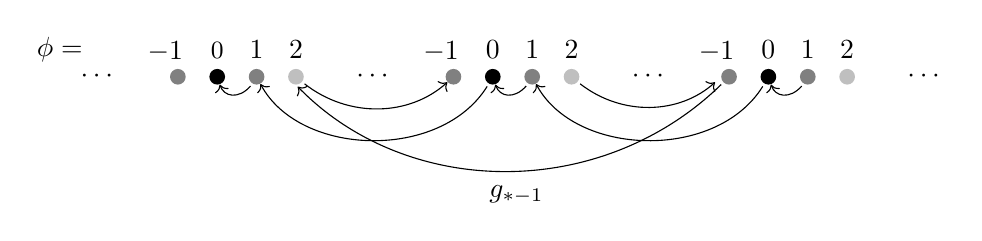
\begin{tikzpicture}

\node at (-5,0) {$\cdots$};
\draw (-4,0) node[circle,fill=gray,inner sep=2pt,label={[xshift=-4.5pt, yshift=-1pt]above: $-1$}] {};
\draw (-3.5,0) node[circle,fill,inner sep=2pt,label={[font=\small]above: $0$}] {};
\draw (-3,0) node[circle,fill=gray,inner sep=2pt,label=above: {$1$}] {} edge[->, bend left=60,looseness=1.5,shorten <=1pt,shorten >=3pt] (-3.5,0);
\draw (-2.5,0) node[circle,fill=lightgray,inner sep=2pt,label=above: {$2$}] {} edge[->, bend right=40,shorten <=1pt,shorten >=3pt] (-0.5,0);

\node at (-1.5,0) {$\cdots$};
\draw (-0.5,0) node[circle,fill=gray,inner sep=2pt,label={[xshift=-4.5pt, yshift=-1pt]above: $-1$}] {};
\draw (0,0) node[circle,fill,inner sep=2pt,label=above: {$0$}] {}  edge[->, bend left=60,shorten <=1pt,shorten >=3pt] (-3,0);
\draw (0.5,0) node[circle,fill=gray,inner sep=2pt,label=above: {$1$}] {} edge[->, bend left=60,looseness=1.5,shorten <=1pt,shorten >=3pt] (0,0);
\draw (1,0) node[circle,fill=lightgray,inner sep=2pt,label=above: {$2$}] {}  edge[->, bend right=40,shorten <=1pt,shorten >=3pt] (2.9,0);
\node at (2,0) {$\cdots$};

\draw (3,0) node[circle,fill=gray,inner sep=2pt,label={[xshift=-4.5pt, yshift=-1pt]above: $-1$}] {} edge[->, bend left=45,shorten <=1pt,shorten >=5pt] (-2.6,0);
\draw (3.5,0) node[circle,fill,inner sep=2pt,label=above: {$0$}] {} edge[->, bend left=60,shorten <=1pt,shorten >=3pt] (0.5,0);
\draw (4,0) node[circle,fill=gray,inner sep=2pt,label=above: {$1$}] {} edge[->, bend left=60,looseness=1.5,shorten <=1pt,shorten >=3pt] (3.5,0);
\draw (4.5,0) node[circle,fill=lightgray,inner sep=2pt,label=above: {$2$}] {};
\node at (5.5,0) {$\cdots$};

\node at (-5.5,0.35) {$\phi=$};
\node at (0.3,-1.5) {$g_{*-1}$};

\end{tikzpicture}
\end{center}

Now, by sending an upper set of $I \in O(\mathbb{Z})$ to its characteristic function $\chi_I$ we get an embedding $$O(\mathbb{Z})^{\textnormal{op}} \hookrightarrow \Xi$$ and the t-structure coming from $(g_{\chi_I})_{\textnormal{\Libra}}(\mathscr{Q})$ is just the tilting of $\mathfrak{t}$ with respect to the torsion pair coming from $I$. \\
The following proposition gives a characterization of the new heart obtained by the above construction. In the case of a mixed filtration, we get a splitting property which is often referred as 'decomposition theorem for perverse sheaves' in literature. \\

\begin{prop}
Let $\mathfrak{t}$ be a bounded t-structure on $\mathscr{D}$, $\mathscr{P}$ a grading filtration on $\heartsuit_{\mathfrak{t}}$, $\mathscr{Q}$ the associated $\mathbb{Z} \ltimes \hat{\mathbb{Z}}$-slicing on $\mathscr{D}$, $p$ a perversity. Denote $\mathfrak{q}$ the bounded t-structure associated to $(g_p)_{\textnormal{\Libra}}(\mathscr{Q})$. Then $\heartsuit_{\mathfrak{q}}$ consists of objects $X \in \mathscr{D}$ so that $$H_{\mathfrak{t}}^{k}(X) \in \mathscr{P}_{p^{-1}(-k)}[k]$$ 
for each $k \in \mathbb{Z}$. Moreover, if $\mathscr{P}$ is a mixed filtration then for each $X \in \heartsuit_{\mathfrak{q}}$ $$X=\bigoplus_{n \in \mathbb{Z}}H_{\mathfrak{t}}^{n}(X)$$ 
\end{prop}

\begin{proof}
This is very similar to \hyperref[tilt1]{\textbf{Proposition \ref*{tilt1}}}: we have that $X \in \heartsuit_{\mathfrak{q}}$ if and only if $$H_{\mathscr{P}}^{\phi}(H_{\mathfrak{t}}^k(X)[-k])[k]=H_{\mathscr{Q}}^{(k,\phi)}(X)=0$$ 
for $p(\phi) \not = -k$. \\
For the second part of the claim, the abelian $\mathbb{Z}$-slicing induced on $\heartsuit_{\mathfrak{q}}$ is split by \hyperref[grad]{\textbf{Proposition \ref*{grad}}} and thus by \hyperref[split]{\textbf{Proposition \ref*{split}}} $$X=\bigoplus_{(k,\phi)}H_{\mathscr{Q}}^{(k,\phi)}(X)=\bigoplus_{n \in \mathbb{Z}}H_{\mathfrak{t}}^{n}(X)$$
where the last equality comes from the first part. 
\end{proof}

\begin{exmp}
Let $$B=\bigoplus_{i\in \mathbb{N}}B_i$$ be an $\mathbb{N}$-graded ring with $B_0$ semisimple. Denote $\mathscr{A}$ the category of $\mathbb{Z}$-graded $B$-modules with only finitely many nonzero graded pieces. For $\phi \in \mathbb{Z}$, denote $\mathscr{P}_{\phi}$ the full subcategory of $\mathscr{A}$ of modules concentrated in degree $\phi$. Clearly, $\mathscr{P}$ defines an abelian $\mathbb{Z}$-slicing on $\mathscr{A}$. Following \cite{kos} we have $$\textnormal{Ext}_{\mathscr{A}}^n(\mathscr{P}_{\phi},\mathscr{P}_{\psi})=0$$
for $n>\psi - \phi$. This means that $\mathscr{P}$ is a mixed filtration and the bounded t-structure on $\mathscr{D}^b(\mathscr{A})$ associated to $(g_1)_{\textnormal{\Libra}}(\mathscr{Q})$ (where $1$ is the identity of $\mathbb{Z}$) is the 'diagonal' (or 'geometric') t-structure which appears in Koszul duality and other areas. 
\end{exmp}

\begin{exmp}
Let $M$ be an $n$-dimensional smooth complex projective variety and consider the $n$-torsion pair $\mathscr{P}$ on $\textnormal{Coh}(M)$ from \hyperref[cohh]{\textbf{Example \ref*{cohh}}}. Using Serre duality and the Grothendieck vanishing theorem, one sees that $\mathscr{P}$, seen as an abelian $\mathbb{Z}$-slicing via the inclusion $[n] \subseteq \mathbb{Z}$, is a perverse filtration. The bounded t-structure associated to $(f_p)_{\textnormal{\Libra}}(\mathscr{Q})$ is the one of perverse coherent sheaves as constructed in \cite{bez}. Following again the proof of \hyperref[t]{\textbf{Proposition \ref*{t}}}, we can use the Harder-Narasimhan filtrations from Gieseker stability to obtain an abelian $J_n$-slicing on the heart of perverse coherent sheaves as done in \cite{perpol}. 
\end{exmp}


{\Huge Da qui in poi ci sono cose gi\`a riportate nella parte sistemata. Le lascio commentate nel file.} 

%\begin{rem} 
%We can give $\per(J)$ the structure of a $\Z$-poset via the incluion $\per(J) \subseteq \pos(\Z,\Oo(J)^\op)$. In general, it will not be totally ordered. However, by taking joins and meets pointwise $\per(J)$ becomes a distributive lattice. 
%\end{rem}
%
%\begin{rem}
%Considering the obvious isomoprhism $\Z \simeq \Oo(\Z)^\op$ a perversity over $\mathbb{Z}$ is just a \textit{monotone and comonotope perversity} in the sense of {\color{red} referenza, tipo bezrukavnikov o BBD}. 
%\end{rem}
%%\begin{prop}\label{pipp}
%%Let $J \overset{f}{\longrightarrow} J'$ be a a $\mathbb{Z}$-equivariant map (not necessarily increasing) between $\mathbb{Z}$-posets, $\mathscr{P}$ a $J$-slicing on $\mathscr{D}$. Suppose that $\mathscr{P}_{\psi} \subseteq \mathscr{P}_{\phi}^{\perp}$ whenever one of the following conditions holds: 
%%\begin{enumerate}[label=(\alph*)]
%%\item $f(\phi) > f(\psi)$
%%\item $f(\phi) + 1 > f(\psi)$ and $\phi +1 < \psi$
%%\end{enumerate}
%%Then $$(f_{\textnormal{\Libra}}(\mathscr{P}))_{\phi}=\mathscr{P}_{f^{-1}(\phi)}$$
%%defines a $J'$-slicing on $\mathscr{D}$.
%%\end{prop}
%%
%%\begin{proof}
%%Part \textit{(1)} of definition of slicing follows from $\mathbb{Z}$-equivariance of $f$, while part \textit{(2)} follows from condition \textit{(a)} above. Pick $0 \not = X \in \mathscr{D}$ and consider its Postnikov tower with respect to $\mathscr{P}$: $$0=Y_0 \overset{\beta_1}{\longrightarrow} \cdots \overset{\beta_n}{\longrightarrow} Y_n=X$$
%%with $\textnormal{cone}(\beta_i)=H_{\mathscr{P}}^{\phi_i}(X)$. Going from left to right, if we encounter an $i$ so that $f(\phi_{i+1}) > f(\phi_i)$ then by condition \textit{(b)} $$\textnormal{Hom}_{\mathscr{D}}(H_{\mathscr{P}}^{\phi_{i+1}}(X),H_{\mathscr{P}}^{\phi_i}(X)[1])=0$$
%%
%%Using \hyperref[g]{\textbf{Proposition \ref*{g}}} and the \hyperref[s]{\textbf{$3 \times 3$ Lemma}}, we can complete the identity of $Y_i$ to get a diagram: 
%%\begin{center}
%%\begin{tikzcd}[ampersand replacement=\&]
%%H_{\mathscr{P}}^{\phi_{i+1}}(X)[-1] \arrow{r} \arrow{d} \& Y_i \arrow{r} \arrow{d}{1} \& Y_{i+1} \arrow{r} \arrow{d} \& H_{\mathscr{P}}^{\phi_{i+1}}(X)[1]\arrow{d} \\
%%Y_{i-1} \arrow{d} \arrow{r} \& Y_i \arrow{r} \arrow{d} \& H_{\mathscr{P}}^{\phi_i}(X) \arrow{r} \arrow{d} \& Y_{i-1}[1] \arrow{d} \\
%%A \arrow{r} \arrow{d} \& 0 \arrow{r} \arrow{d} \& A[1] \arrow{r} \arrow{d} \& A[1] \arrow{d}  \\
%%H_{\mathscr{P}}^{\phi_{i+1}}(X) \arrow{r}  \&  Y_i[1] \arrow{r} \& Y_{i+1}[1] \arrow{r} \&  H_{\mathscr{P}}^{\phi_{i+1}}(X)[1]
%%\end{tikzcd}
%%\end{center}
%%
%%We then replace $\beta_i$ with $Y_{i-1} \longrightarrow A$ and $\beta_{i+1}$ with $A \longrightarrow Y_{i+1}$. Iterating this process\footnote{This is somehow reminiscent of the 'bubble sort' algorithm.}, we get a factorization $$0=Z_0 \overset{\gamma_1}{\longrightarrow} \cdots \overset{\gamma_n}{\longrightarrow} Z_n=X$$
%%with $\textnormal{cone}(\gamma_i)=H_{\mathscr{P}}^{\phi_{k_i}}(X)$ for some $k_i$ and $f(\phi_i) \ge f(\phi_{i+1})$ for all $i$. To get a factorization with the strict latter inequality we use the same argument as in the proof of \hyperref[af]{\textbf{Proposition \ref*{af}}}.
%%\end{proof}
%%
%%The above proof also shows that, in the same hypotheses and notation, $(f_{\textnormal{\Libra}}(\mathscr{P}))_{\phi}$ consists of objects $X \in \mathscr{D}$ so that $H_{\mathscr{P}}^{\psi}(X)=0$ for $ f(\psi) \not = \phi$. Also, \hyperref[aae]{\textbf{Proposition \ref*{aae}}} holds when $f$ is bijective.\\
%
%%\begin{defn}
%%A map $\mathbb{Z} \overset{p}{\longrightarrow} \mathbb{Z}$ is called \textbf{perversity} if it is a monotone contraction, i.e. if $$0 \le p(\phi) - p(\psi) \le \phi - \psi$$ 
%%whenever $\phi \ge \psi$  in $\mathbb{Z}$. \\
%%We denote $\Xi$ the set of perversities. 
%%\end{defn}
%%
%%Clearly, $\Xi$ definies a $\mathbb{Z}$-poset which is not totally ordered. However, it is a distributive lattice: we have meets and joins given by: $$(p\land q)(\phi)=\min\{p(\phi), q(\phi) \}$$ $$(p\lor q)(\phi)=\max\{p(\phi), q(\phi) \}$$
%%Indeed, if we place on $\mathbb{Z}\times \mathbb{Z}$ the product order, we have an isomorphism of $\mathbb{Z}$-posets $$\Xi^{\textnormal{op}}=O(\mathbb{Z}\times \mathbb{Z})\setminus \{ \emptyset, \mathbb{Z} \times \mathbb{Z} \} $$
%%given by sending the zero perversity to $A=\{ (\phi,\psi) \}_{\phi \ge 0} $ and the identity to $B=\{ (\phi,\psi) \}_{\psi \ge 0}$ ($B+i$ and $A+i$ with $i \in \mathbb{Z}$ generate the latter as a complete lattice). Considering the canonical embedding $\mathbb{Z} \hookrightarrow \mathbb{Z}  \subseteq O(\mathbb{Z} \times \mathbb{Z})$ we get a sublattice of $\Xi$ depicted as 
%%
%% \begin{center}
%%      \begin{tikzpicture}
%%        \draw (-2,-2) -- (-1,-1) -- (0,0) -- (1,-1) -- (2,-2);
%%        \draw (-1,-1) -- (0,-2) -- (1,-1);
%%        \draw (-3,-3) -- (-2,-2) -- (-1,-3) -- (0,-2) -- (1,-3) -- (2,-2) -- (3,-3);
%%       \node at (0,1) {$\vdots$};
%%       \node[circle, draw, fill=black, inner sep=0pt, minimum width=4pt] at (0,0) {};
%%       \node[circle, draw, fill=black!50, inner sep=0pt, minimum width=4pt] at (-1,-1) {};
%%       \node[circle, draw, fill=black!50, inner sep=0pt, minimum width=4pt] at (1,-1) {};
%%       \node[circle, draw, fill=black!50, inner sep=0pt, minimum width=4pt] at (0,-2) {};
%%       \node[circle, draw, fill=black!50, inner sep=0pt, minimum width=4pt] at (-2,-2) {};
%%       \node[circle, draw, fill=black!50, inner sep=0pt, minimum width=4pt] at (2,-2) {};
%%       \node[circle, draw, fill=black!50, inner sep=0pt, minimum width=4pt] at (-3,-3) {};
%%       \node[circle, draw, fill=black!50, inner sep=0pt, minimum width=4pt] at (-1,-3) {};
%%       \node[circle, draw, fill=black!50, inner sep=0pt, minimum width=4pt] at (1,-3) {};
%%       \node[circle, draw, fill=black!50, inner sep=0pt, minimum width=4pt] at (3,-3) {};
%%       \node at (0,-4) {$\vdots$};
%%      \end{tikzpicture}
%%    \end{center}
%%This induces the 't-tree' described in \cite{matti}, as discussed below in a far-reaching generality. By the other hand, each square above contains moreover a copy of the Young lattice
%% \begin{center}
%%      \begin{tikzpicture}[nodes={circle, draw, fill=black!50, inner sep=0pt, minimum width=4pt}]
%%              \draw (2,-4) -- (1.5,-3) -- (1,-2) -- (0.5,-1) -- (0,0) -- (-0.5,-1) -- (-1,-2) -- (-1.5,-3) -- (-2,-4);
%%        \draw (1.5,-3) -- (1.5,-4) -- (0.75,-3) -- (0,-2) -- (-0.75,-3) -- (-1.5,-4) -- (-1.5,-3);
%%        \draw  (1,-4) -- (0.75,-3) -- (0.5,-4) -- (0,-3) -- (-0.5,-4) -- (-0.75,-3) -- (-1,-4);
%%        \draw (0,-3) -- (0,-2);
%%        \draw (0.5,-1) -- (0,-2) -- (-0.5,-1);
%%        \draw (-0.75,-3) -- (-1,-2);
%%        \draw (0.75,-3) -- (1,-2);
%%        \draw (0,1) -- (0,0);
%%        \node[fill=black] at (0,1) {};
%%        \node at (0,0) {};
%%        \node at (-0.5,-1) {};
%%        \node at (0.5,-1) {};
%%        \node at (0,-2) {};
%%        \node at (1,-2) {};
%%        \node at (-1,-2) {};
%%        \node at (0,-3) {};
%%        \node at (0.75,-3) {};
%%        \node at (-0.75,-3) {};
%%        \node at (1.5,-3) {};
%%        \node at (-1.5,-3) {};
%%        \node at (-2,-4) {};
%%        \node at (-1.5,-4) {};
%%        \node at (-1,-4) {};
%%        \node at (-0.5,-4) {};
%%        \node at (0.5,-4) {};
%%        \node at (1,-4) {};
%%        \node at (1.5,-4) {};
%%        \node at (2,-4) {};
%%        \node[draw=none, fill=white] at (0,-5) {$\vdots$};
%%      \end{tikzpicture}
%%    \end{center}
%%
%%with the root corresponding to the upper vertex of the square. 
%
%\begin{prop}\label{grad}
%Let $\mathfrak{t}$ be a bounded t-structure on $\mathscr{D}$, $\mathscr{P}$ an abelian $\mathbb{Z}$-slicing on $\heartsuit_{\mathfrak{t}}$, $\mathscr{Q}$ the associated $\mathbb{Z} \ltimes \hat{\mathbb{Z}}$-slicing on $\mathscr{D}$, $p$ a perversity. We have: 
%\begin{enumerate}
%\item if $\mathscr{P}$ is a perverse filtration, then $\mathscr{Q}$ satisfies the assumptions of \hyperref[pipp]{\textbf{Proposition \ref*{pipp}}} with respect to the map $\mathbb{Z} \ltimes \hat{\mathbb{Z}} \overset{f_p}{\longrightarrow} \mathbb{Z} \ltimes \hat{\mathbb{Z}}$ given by $$f_p(n,\phi)=(n+p(\lfloor \phi / 2 \rfloor),-p(\lfloor \phi / 2 \rfloor))$$ 
%\item if $\mathscr{P}$ is a grading filtration, then $\mathscr{Q}$ satisfies the assumptions of \hyperref[pipp]{\textbf{Proposition \ref*{pipp}}} with respect to the map $\mathbb{Z} \ltimes \hat{\mathbb{Z}} \overset{g_p}{\longrightarrow} \mathbb{Z} \ltimes \hat{\mathbb{Z}}$ given by $$g_p(n,\phi)=(n+p(\phi),-p(\phi))$$ 
%\item if $\mathscr{P}$ is a mixed filtration, then the abelian $\mathbb{Z}$-slicing induced on the heart of the bounded t-structure associated to $(g_p)_{\textnormal{\Libra}}(\mathscr{Q})$ is split 
%\end{enumerate}
%\end{prop}
%
%\begin{proof}
%Let's prove \textit{(2)}. Suppose $g_p(n,\phi) > g_p(m,\psi)$. Then either $m-n< p(\phi) - p(\psi)$ or both $m-n = p(\phi) - p(\psi)$ and $p(\psi) < p(\psi)$. Since by definition of t-structure we can assume $m \ge n$, the second case is absurd while in the first case, since $p$ is monotone, we have $\phi \ge \psi$ and thus by definition of perversity $$m-n<p(\phi)-p(\psi) \le \phi - \psi$$ 
%and we get the desired Hom-vanishing by definition of grading filtration. \\
%
%Suppose now $f_p(n,\phi) + 1 > f_p(m,\psi)$ and $(n+1,\phi) < (m,\psi)$. The only non absurd case is $ 1<m-n \le  p(\phi) - p(\psi)$. But then again we have $$2 \le m-n \le p(\phi)-p(\psi) \le \phi - \psi$$
%and we can conclude as above. \\
%
%To prove \textit{(1)} consider the monotone map $$\mathbb{Z} \overset{\lfloor * / 2 \rfloor}{\longrightarrow} \mathbb{Z}$$
%Applying the slice functor to the latter and starting with a perverse filtration, we get a grading filtration by the properties of the floor function and the thesis follows from part \textit{(2)}. \\ 
%
%Let's prove \textit{(3)}. We have to show that $$\mathscr{P}_{\psi}[1-p(\psi)] \subseteq \mathscr{P}_{\phi }[p(\phi)]^{\perp}$$ 
%for $-p(\psi)>-p(\phi)$. We denote $n=p(\phi)-p(\psi)-1$. Assuming again $n \ge 0$, we have $n \ge 0 > p(\psi) - p(\phi) \ge \psi - \phi$ and we can then conclude by definition of mixed filtration. 
%\end{proof}
%
%

%
%Now we somehow review the gluing construction for t-structures in \cite{del}, but generalize it to any slicing. Our language is quite different though, and we formulate the problem very similarly to \cite{glu}. We start with two $\mathbb{Z}$-posets $J,J'$. 
%
%\begin{defn}
%Let $\mathscr{P}$ be a $J \ltimes J'$-slicing on $\mathscr{D}$. We call $\mathscr{P}$ \textbf{gluable} if it satisties the assumptions of \hyperref[pipp]{\textbf{Proposition \ref*{pipp}}} with respect to the map $J \ltimes J' \overset{e}{\longrightarrow} J' \ltimes J$ that exchanges coordinates. In this case we denote $$\overline{\mathscr{P}}=e_{\textnormal{\Libra}}(\mathscr{P})$$
%\end{defn}
%
%By a simple computation, the gluability condition reads: $\mathscr{P}_{(\phi,\psi)} \subseteq \mathscr{P}_{(\phi',\psi')}^{\perp}$ if $\psi' > \psi$ or both $\psi'+1>\psi$ and $\phi'+1 < \phi$. For example, the first condition is automatic when $\mathbb{Z}$ acts trivially on $J$ (in this case, it follows from the second one). In particular, if $\mathbb{Z}$ acts trivially on $J$, $\mathscr{P}$ is a $J$-slicing on $\mathscr{D}$ and $\mathfrak{t}_{\phi}$ is a bounded t-structure on $\mathscr{P}_{\phi}$ for each $\phi \in J$, then using \hyperref[aab]{\textbf{Proposition \ref*{aab}}} we get a $J \ltimes \mathbb{Z}$-slicing $\mathscr{Q}$ which is gluable if and only if $$\heartsuit_{\mathfrak{t}_{\psi}}[n] \subseteq \heartsuit_{\mathfrak{t}_{\phi}}^{\perp}$$
%whenever both $n \le 0$ and $\phi < \psi$. 
%
%\begin{rem}
%We have a commutative diagram of $\mathbb{Z}$-posets 
%\begin{center}
%\begin{tikzcd}[ampersand replacement=\&]
%\mathbb{Z} \ltimes \mathbb{Z} \arrow{r}{\sim} \arrow{d}{e} \& \mathbb{Z} \ltimes \hat{\mathbb{Z}} \arrow{d}{g} \\
%\mathbb{Z} \ltimes \mathbb{Z} \arrow{r}{\sim}  \& \mathbb{Z} \ltimes \hat{\mathbb{Z}} 
%\end{tikzcd}
%\end{center}
%where the horizontal isomorphism is the one from \hyperref[zet]{\textbf{Remark \ref*{zet}}}. Indeed, a $\mathbb{Z} \ltimes \mathbb{Z}$-slicing on $\mathscr{D}$ is gluable if and only if it induces a grading filtration on the heart of the associated t-structure when seen as a $\mathbb{Z} \ltimes \hat{\mathbb{Z}}$-slicing. 
%\end{rem} 
%
%An easy combinatorial calculation finally yelds the following two remarks: 
%\begin{itemize}
%\item  if $\mathscr{P}$ is a gluable $\hat{\mathbb{Z}} \ltimes \mathbb{Z}$-slicing on $\mathscr{D}$, then $\overline{\mathscr{P}}$ induces a grading filtration on the associated heart, allowing us again to construct new bounded t-structures depending on a perversity. 
%\item if $\mathscr{P}$ is a mixed filtration on the heart of a bounded t-structure and $\mathscr{Q}$ is the associated $\mathbb{Z} \ltimes \hat{\mathbb{Z}}$-slicing on $\mathscr{D}$, then $\mathscr{Q}$ is gluable. In this case, looking at $\overline{\mathscr{Q}}$, we get a baric structure on $\mathscr{D}$ which is usually called \textbf{weight decomposition} in literature. 
%\end{itemize}
%In other words, the chain of implications for a $\mathbb{Z} \ltimes \hat{\mathbb{Z}}$-slicing refines to 
%$$\textnormal{mixed} \implies \textnormal{gluable} \implies \textnormal{grading} \implies \textnormal{perverse} $$
%
%%\begin{prop}
%%A $J \ltimes J'$-slicing $\mathscr{P}$ on $\mathscr{D}$ is gluable if and only if it satifies the assumptions of \hyperref[pipp]{\textbf{Proposition \ref*{pipp}}} with respect to the identity (as sets) $J \ltimes J' \longrightarrow J \times J'$, where we place the product order on the right member. 
%%\end{prop}
%%
%%\begin{proof}
% % Consider the following commutative diagram of sets
% % \begin{center}
%%\begin{tikzcd}[ampersand replacement=\&]
%%J \ltimes J' \arrow{r}{e} \arrow{d}{1} \& J \ltimes J' \\
%%J \times J' \arrow{r}{e}  \& J \times J' \arrow{u}{1}
%%\end{tikzcd}
%%  \end{center}
%%  The right arrow is a morphism of $\mathbb{Z}$-posets while the down one is an isomorphism of $\mathbb{Z}$-posets, and the thesis follows. 
%%\end{proof}
%%\begin{prop}
%%Let $\mathscr{P}$ be a gluable $J \times J'$-slicing on $\mathscr{D}$. For $i = 1,2$, denote $\mathscr{P}^i=\pi_{\textnormal{\Libra}}^i(\mathscr{P})$, where $J \overset{\pi^1}{\longleftarrow} J \times J' \overset{\pi^2}{\longrightarrow} J'$ are the projections. Then for each $\psi \in J'$, $\mathscr{P}_{\psi}^2$ consists of objects $X \in \mathscr{D}$ so that $$H_{\mathscr{P}^1}^{\phi}(X) \in \mathscr{Q}_{(\phi,\psi)}$$
%%for each $\phi \in J$.
%%\end{prop}
%%
%%\begin{proof}
%%We have already seen that $X \in \mathscr{P}_{\psi}^2$ if and only if $$H_{\mathscr{P}}^{\lambda}(X)=H_{\mathscr{P}}^{\lambda}(H_{\mathscr{P}^1}^{\pi^1(\lambda)}(X))=0$$
%%for $\pi^2(\lambda) \not =\psi$. By fixing $\pi^1(\lambda)=\phi$ and varying $\pi^2(\lambda)$, we get the desired result. 
%%\end{proof}
\newpage



\afterpage{\blankpage}
\clearpage 
\bibliographystyle{alpha}


\end{document}
